% v2-acmsmall-sample.tex, dated March 6 2012
% This is a sample file for ACM small trim journals
%
% Compilation using 'acmsmall.cls' - version 1.3 (March 2012), Aptara Inc.
% (c) 2010 Association for Computing Machinery (ACM)
%
% Questions/Suggestions/Feedback should be addressed to => "acmtexsupport@aptaracorp.com".
% Users can also go through the FAQs available on the journal's submission webpage.
%
% Steps to compile: latex, bibtex, latex latex
%
% For tracking purposes => this is v1.3 - March 2012

\documentclass[prodmode]{acmsmall} % Aptara syntax

\usepackage{pdfpages}
\usepackage{graphicx}
\usepackage{morefloats}
%\usepackage{cite}
%\usepackage[style=numeric, backend=biber, sorting=none]{biblatex}
%\addbibresource{references.bib}
\usepackage{listings}
\lstset{
basicstyle=\small\ttfamily,
columns=fullflexible,
breaklines=true,
%float=H
}

% Document starts
\begin{document}

% Page heads
\markboth{Evan Bradley}{Analysis of 2016 Presidential Election-related Twitter Hashtags}

% Title portion
\title{Analysis of 2016 Presidential Election-related Twitter Hashtags}
\author{
  EVAN BRADLEY
  \affil{Oakland University}
}

\begin{abstract}
  The 2016 presidential election was considered to be one of the most atypical
  elections in the months prior to the election, as well as after. After the
  upset victory of Republican nominee Donald Trump over his opponent, Democratic
  nominee Hillary Clinton, a large social discourse began over the unexpected
  results of the election. As a major online social media platform, Twitter
  found itself at the epicenter of these, with numerous hashtags, a tool used to
  categorize Tweets, emerging as a result of enthusiasm on all sides of the
  political spectrum. A sample of popular hashtags was taken and all known
  tweets posted with these hashtags were collected over the course of a week.
  Using these hashtags as groupings for community, they were observed and
  analyzed as a window into the public discourse in the weeks following the
  election. It was found that the lifetimes of the hashtags could be quite
  short, and that of the hashtags collected, most users identified as supporting
  Trump. This was reflected in further analysis, which suggested that most the
  tweets collected discussed topics related Trump and furthermore were generally
  sympathetic to his views.
\end{abstract}

\keywords{Data mining, Text mining, Twitter, 2016 Presidential Election, Donald Trump}

\maketitle

\section{Introduction} %cite 538 & NYT
The 2016 presidential election resulted in the massive upset victory of Donald
Trump, who was seen in the weeks and days prior to the election to have little
to no chance of winning. Many news outlets casted high predictions that his
opponent, Hillary Clinton, would win the election, with predicted likelihoods of
her victory as high as 98\% \cite{huffpost}. An immediate backlash
followed on Twitter, with the \#NotMyPresident hashtag gaining significant
popularity, leading to riots throughout the United States \cite{riots}. Those
who supported Trump also took to Twitter, congregating on hashtags such as \#MAGA
and \#DrainTheSwamp.

Hashtags were selected as the grouping for data collection for their utility to
Twitter users: they provide a platform for users to converse on a topic with
people whom they do not follow or even necessarily know. They often represent a
core idea that a community wishes to comment on. There are no membership
requirements, so they often attract whichever users are looking to add their
voice to the conversation. Because of their communal nature, each hashtag was
analyzed in isolation to gain insights from its users, and to clear up the noise
that would ensue from gathering data over multiple hashtags.

\subsection{Data collection}
Data was collected semi-continuously from November 20 to December 9 through
Twitter's stream API using a Node.js script equipped with the Twit node module.
The stream would accept any new Tweets posted containing that hashtag, which
would be stored in a JSON file for later retrieval. The JSON files contained the
entire tweet object sent by Twitter, and were segmented into files containing a
maximum of 50,000 tweets to allow for easier handling. The stream collected
tweets constantly aside from a few minor interruptions induced by connection
issues. As a result of these and the added hashtags halfway through collection,
some of the analysis has been split between November 20 to November 29 and
December 1 to December 9. The initial hashtags were collected throughout the
collection process, but the set of newer hashtags was only collected in the
second time window.

The hashtags originally chosen for collection were \#Election2016,
\#NotMyPresident, and \#ElectionNight. These were
chosen for their perceived popularity and relevance to the topic. However, the
hashtags grew less popular as collection continued, and so new hashtags were
added on November 31 to increase the number of tweets available for mining. These
were \#Trump, \#Clinton, \#MakeAmericaGreatAgain, \#MAGA, and \#DrainTheSwamp.
\#Trump and \#Clinton served as mostly neutral tags, with a mixture of
discussion from both supporters and non-supporters of each candidate. The
remaining three hashtags were largely used by Trump supporters, with ``Make
America Great Again'' being Trump's campaign slogan, and ``Drain the Swamp'' a
phrase he often used to refer to one of his proposed policies once in office.
These largely picked up in activity where the other tweets were dwindling, and
were able to offer more insight about public opinion in the weeks following the
election.

\subsection{Data Pre-processing}
While Twitter is frequently a great source for researchers as a source for
public opinion, the contents of tweet objects often vary a great deal in format
and thus require a considerable amount of pre-processing. The collected tweets
were processed using another Node.js script, which would perform a number of
tasks to prepare them in a palatable form for analysis in R.

The Node.js script's chief task was to extract data in the tweet objects deemed
as useful for text mining and write it to a CSV file would then be easily read
into R. The script starts by reading in data from a specified numbered data file
containing a JSON object with the desired tweets. This object is unable to fit
into memory, so the tweets are read in by line from the JSON object, where they
are sent to be processed and placed in the proper CSV file.

The preprocessing begins by writing the tweet's timestamp in a format that can
be more easily parsed, and continues to strip hashtags and emoji from the
tweet's text, which are placed into their own columns for analysis. The text is
heavily processed to remove links and various characters to ensure no issues are
encountered when the data is read into R. The retweet status, user biographical
information, and self-written user location are also placed into the CSV file
alongside the rest of the tweet information. Each tweet is written into a
separate CSV file that contains all tweets of a common selected hashtag. Tweets
containing two selected hashtags are placed into two files, for analysis within
other tweets of each of those hashtags.

\begin{table}[!t]
  \tbl{Description of the variables selection from the tweets for further analysis.}{
  \begin{tabular}{ | c | c | }
\hline
    \textbf{Name of variable} & \textbf{Description} \\ \hline
    time & Timestamp including date and time \\ \hline
    hashtags & Other hashtags included in the tweet \\ \hline
    emoji & Any emoji used in the tweet \\ \hline
    text & The tweet itself \\ \hline
    bio & The user's self-written biography \\ \hline
  \end{tabular}}
\end{table}

The decision to place the same tweet into multiple files (and thus duplicate it)
is rationalized by that it is impossible to determine what the ``main'' hashtag
of the tweet is, so it would be best to duplicate it for analysis as part of
both. As communities, hashtags can also interact with each other, so analyzing
the same tweet as a part of both hashtags would be the best method to capture
this interaction.

Closely related is the decision to keep retweets in the data and perform
analysis on them. As complete repeats of other tweets, it may seem sensible to
remove re-tweets, but considering the brief, 140-character limit on tweets, it
may seem enticing to many users to simply repeat what another user has said. To
this effect, a retweet can be seen as constituting two people saying the exact
same thing, which can be useful in situations such as sentiment analysis, which
attempts to aggregate this data from the whole.

\section{Hashtag Trends}
Before analyzing the data any further, the tweets in each hashtag group were
aggregated over time to observe the trend of their popularity over the week they
were collected. The tweet counts were graphed using a histogram with 12-hour
bins to time the aggregation of the tweets. These aggregations were then plotted
using \verb|ggplot2|, with different colors representing the popularity of the
hashtag during that interval. The first batch of tweet collection was performed
from November 20 to November 29 on the \#Election2016, \#ElectionNight, and
\#NotMyPresident hashtags.

As would be expected of event-specific hashtags, the \#Election2016 and
\#ElectionNight hashtags were relatively unpopular two weeks after the election
itself, only accumulating less than 8,000 tweets a day each. Most of these
tweets are unlikely to only contain their hashtag, but instead tag along with
other hashtags in an effort by the user to reach a wider audience, or to simply
include the event in their tweet even if it isn't the primary subject. Both
hashtags also became even less frequent over the week, though still registering
at over 2,000 tweets a day.
 
The \#NotMyPresident tweet maintained considerably more popularity, starting off
at roughly 20,000 tweets a day at its height and around 8,000 tweets a day at
its low point. It also showed signs of declining popularity, suggesting either
fatigue amongst its supporters or a shift in topic to another hashtag.
Regardless, these numbers are likely considerably lower than they were
immediately after the election, definitively indicating a change in the
conversation as time went on.

\begin{figure*}
\centering
\begin{minipage}[b]{.49\textwidth}
    \includegraphics[width = \textwidth]{set1/freq-election2016}
\caption{The election-specific hashtags both shared a relatively low throughput
  with further downward trends in usage.}\label{election chart}
\end{minipage}\hfill
\begin{minipage}[b]{.49\textwidth}
    \includegraphics[width = \textwidth]{set1/freq-notmypresident}
\caption{The opposition to Trump maintained a portion of its original popularity
  after the election, but also showed signs of either fatigue or a shift.}
\label{notmypresident chart}
\end{minipage}
\end{figure*}

From December 1 to December 9, the \#AmericaFirst, \#Clinton, \#DrainTheSwamp,
\#MAGA, \#MakeAmericaGreatAgain, and \#Trump hashtags were added to the list of
hashtags to be collected to gain more insights about post-election public
opinion. Collection continued on the first three hashtags to observe how they
fared further away from the election.

The \#Election2016 and \#ElectionNight hashtags continued their decline, halving
their tweets per day from the previous collection window. \#Election2016 saw
roughly 2,000 tweets per day while \#ElectionNight saw under 1,000 tweets per
day, and both showed signs of further declining despite a spike around December
7-8. The \#NotMyPresident hashtag also declined further, now declining to under
8,000 tweets per day.

Some of the newer hashtags fared considerably better than those in the first
set, while some garnered a similar number of tweets per day. The least used
hashtags were \#Clinton, \#DrainTheSwamp, \#MakeAmericaGreatAgain, and
\#AmericaFirst, which saw roughly 1,000, 4,000, under 10,000, and roughly 10,000
tweets per day, respectively. The \#Clinton and \#DrainTheSwamp hashtags saw no
discernible trend, maintaining a roughly even number of tweets per day
throughout the week. \#AmericaFirst showed signs of a slow decrease in its tweet
count, declining from a 30,000 tweet spike to roughly 8,000 tweets per day.
\#MakeAmericaGreatAgain saw a steady decline during the first half of the
collection window before a sudden spike on December 6, followed by another
steady decrease off of the increased numbers caused by the spike.

\begin{figure*}
\centering
\begin{minipage}[b]{.49\textwidth}
    \includegraphics[width = \textwidth]{set2/freq-americafirst}
\caption{Most of the pro-Trump hashtags collected saw signs of fatigue over the
  collection window.}\label{americafirst chart}
\end{minipage}\hfill
\begin{minipage}[b]{.49\textwidth}
    \includegraphics[width = \textwidth]{set2/freq-maga}
\caption{The MAGA hashtag was by far the most tweeted hashtag collected,
  likely due to its generality in meaning.}
\label{maga chart}
\end{minipage}
\end{figure*}

The \#Trump and \#MAGA hashtags saw the greatest number of tweets collected in
both windows, and throughout the collection window showed no signs of decrease.
\#Trump and \#MAGA had roughly 40,000 and 80,000 tweets respectively,
accounting for numbers an order of magnitude larger than the rest of the tweets.
This points to a very active and engaged base of Trump supporters on Twitter as
well as a need for more sophisticated methods in choosing popular hashtags from
which to collect tweets.

\section{Hashtag Users}
To determine the general disposition of users tweeting on the collected
hashtags, the biographical information of each user in each tweet was mapped to
a word cloud for easy visualization. To accomplish this, duplicate user
biographies were removed to account for users posting on the same hashtag
multiple times. The strings consisting of the biographies were then further
cleaned and fed into a term-document matrix. Terms that appeared in a
significant portion of user biographies were then taken and mapped to the
wordcloud using the \verb|wordcloud| library.

Analysis of the user biographies of the hashtags revealed that the majority of
users in the sampled hashtags identified as conservative Trump supporters. This
came as a bit of a surprise, since the expected demographic of Twitter users is
typically young, liberal millenials. With all hashtags but the \#NotMyPresident
hashtag, however, the terms users used in their biographies were nearly
identical for most hashtags. Users identified as conservative Trump supporters
with terms such as ``god'', ``christian'', and ``maga'' appearing frequently in
all biographies. It is unclear whether this indicates the same users appearing
across the different hashtags, but it does indicate that whoever is using the
hashtags is more likely to support Trump than otherwise. Furthermore, the
inclusion of these Terms in their biographies indicates that they are very
politically driven and therefore may not represent average Americans expressing
a view.

\begin{figure*}
\centering
\begin{minipage}[b]{.49\textwidth}
    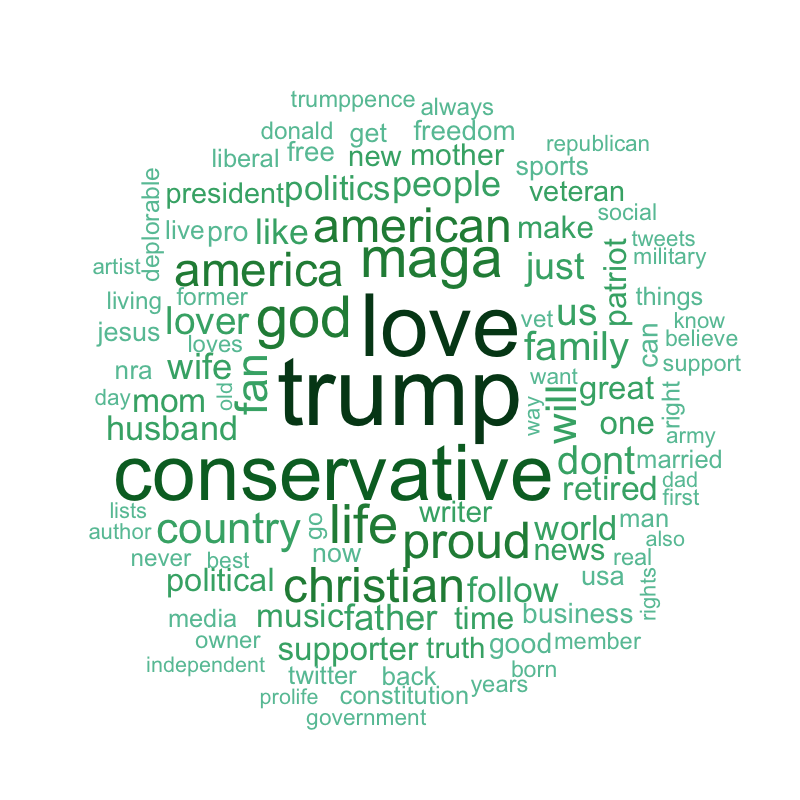
\includegraphics[width = \textwidth]{cloud-maga}
\caption{A wordcloud showing popular terms in users' biographies who tweeted using
  the MAGA hashtag. a majority of the other hashtags looked very
  similar.}\label{maga cloud}
\end{minipage}\hfill
\begin{minipage}[b]{.49\textwidth}
    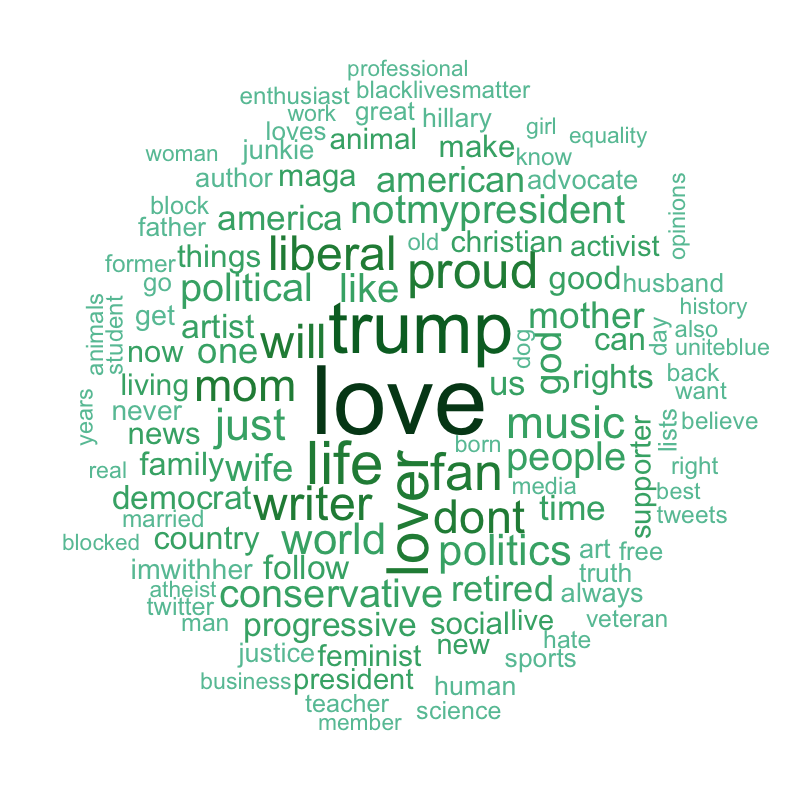
\includegraphics[width = \textwidth]{cloud-notmypresident}
\caption{A wordcloud showing popular terms in users' biographies who tweeted using
  the NotMyPresident hashtag.}\label{notmypresident cloud}
\end{minipage}
\end{figure*}

%\begin{figure}[!t]
%  \tbl{A wordcloud showing popular terms in users' biographies who tweeted using
%  the \#MAGA hashtag. A majority of the other hashtags looked very similar.}{
%    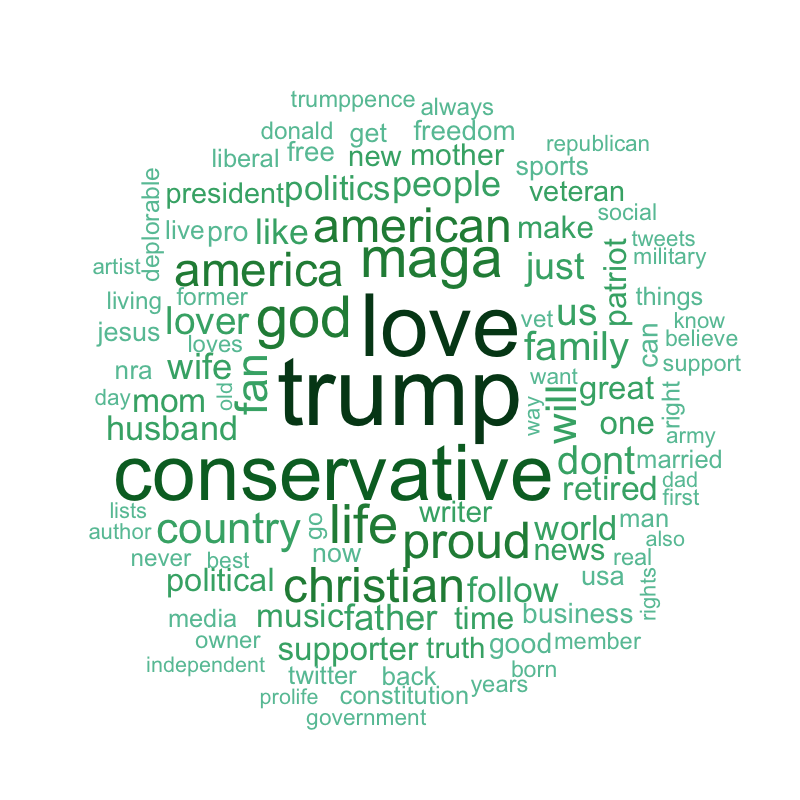
\includegraphics[width = \textwidth]{cloud-maga}}
%\end{figure}

The \#NotMyPresident hashtag, as the sole outlier, included other words in the
user biographies such as ``writer'', ``mom'', ``liberal'', and ``feminist'' that
indicated users on the hashtag were more unlikely to be Trump supporters. This
would be more in line with the popular view of the hashtag, which indicates
those who stand adamantly against Trump on the basis of his actions and views.

%\begin{figure}[!t]
%  \tbl{A wordcloud showing popular terms in users' biographies who tweeted using
%  the \#NotMyPresident hashtag.}{
%    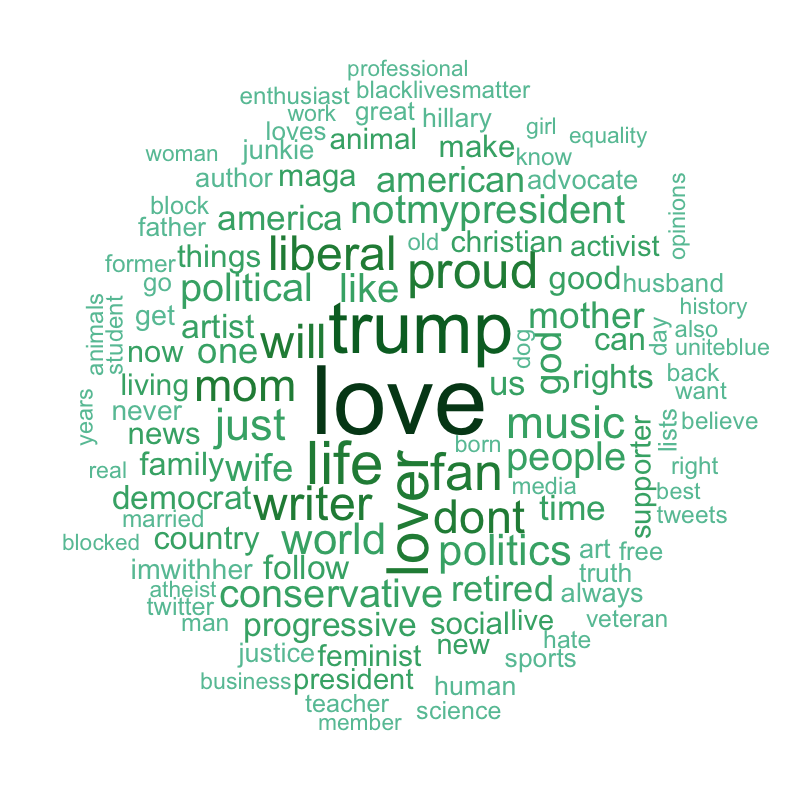
\includegraphics[width = \textwidth]{cloud-notmypresident}}
%\end{figure}
\section{Popular Hashtags Within Hashtags}
To view the relationship between different hashtags and to peer into the related
topics people were discussing, hierarchical clustering was applied to the other
hashtags used on each tweet of a particular ``primary'' hashtag. This was done
by feeding a term-document matrix representation of the text for the hashtags of
the tweet directly into R's \verb|hclust| method, which was then plotted on a
graph. The results were largely in line with what was discovered about the user
base for each hashtag, but did provide for further insights about the sorts of
discussions users were having on each hashtag.

The \#AmericaFirst, \#DrainTheSwamp, \#ElectionNight, \#MakeAmericaGreatAgain,
\#MAGA, and \#Trump hashtags all appeared relatively similar as hashtags that
support Trump by name. Most related hashtags seemed to take a congratulatory
tone on his victory or discuss current news items related to the
president-elect.

\begin{figure*}
\centering
\begin{minipage}[b]{.49\textwidth}
    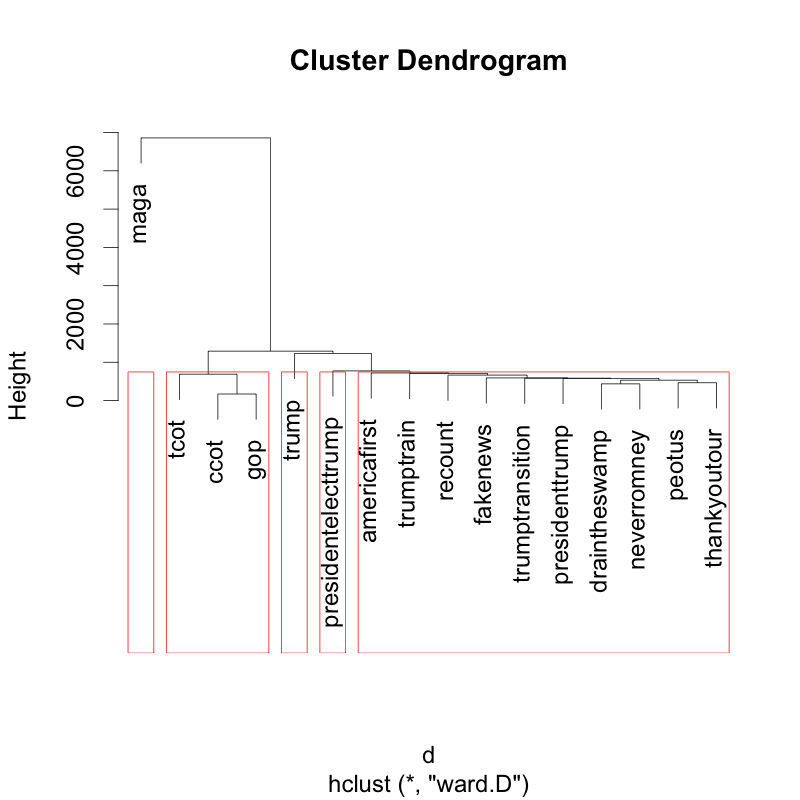
\includegraphics[width = \textwidth]{cluster-maga}
\caption{A hierarchical cluster of hashtags used with the MAGA hashtag. Many
  hashtags listed as related here were also seen in the other primary hashtags.}
\label{maga cluster}
\end{minipage}\hfill
\begin{minipage}[b]{.49\textwidth}
    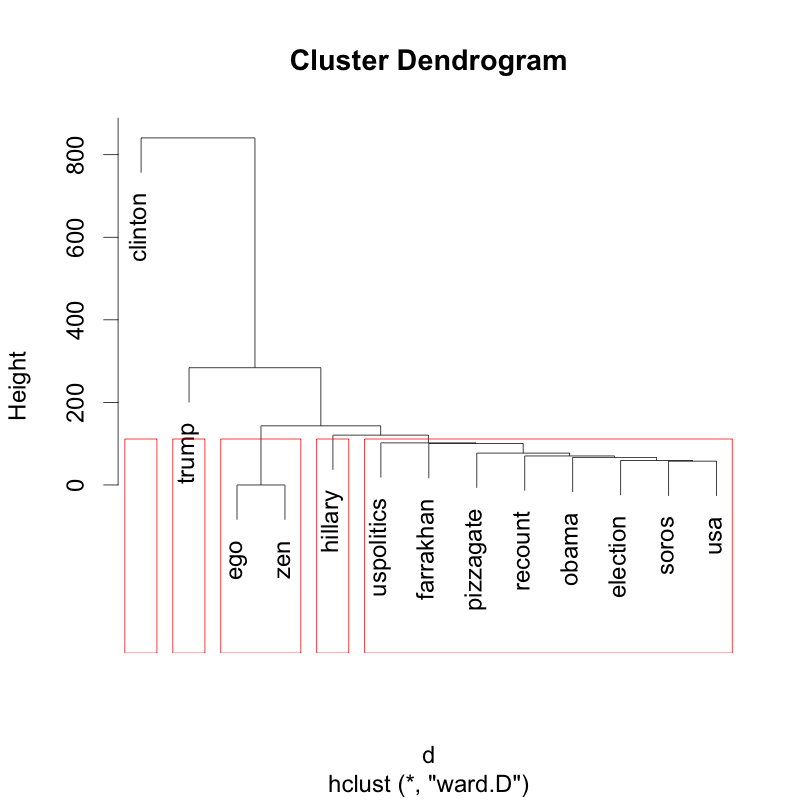
\includegraphics[width = \textwidth]{cluster-clinton}
\caption{A hierarchical cluster of hashtags used with the \#Clinton hashtag.}
\label{clinton cluster}
\end{minipage}
\end{figure*}

The \#Clinton hashtag was more unclear, with a number of hashtags on figures and
news items included relatively often. Of particular note is the frequency with
which the \#Trump hashtag appears with the \#Clinton hashtag, but this happens
to a lesser extent the other way around. This would indicate that tweets on
Clinton are much likely to be discussing her in relation to Trump, as where
Trump is more likely to be discussed on his own.

The \#Election2016 hashtag largely contains more pro-Trump hashtags, but does
show some discontent from non-supporters of Trump, with the \#HillaryClinton,
\#ImStillWithHer, and \#AuditTheVote hashtags appearing in smaller clusters
with the primary hashtag.

\begin{figure*}
\centering
\begin{minipage}[b]{.49\textwidth}
    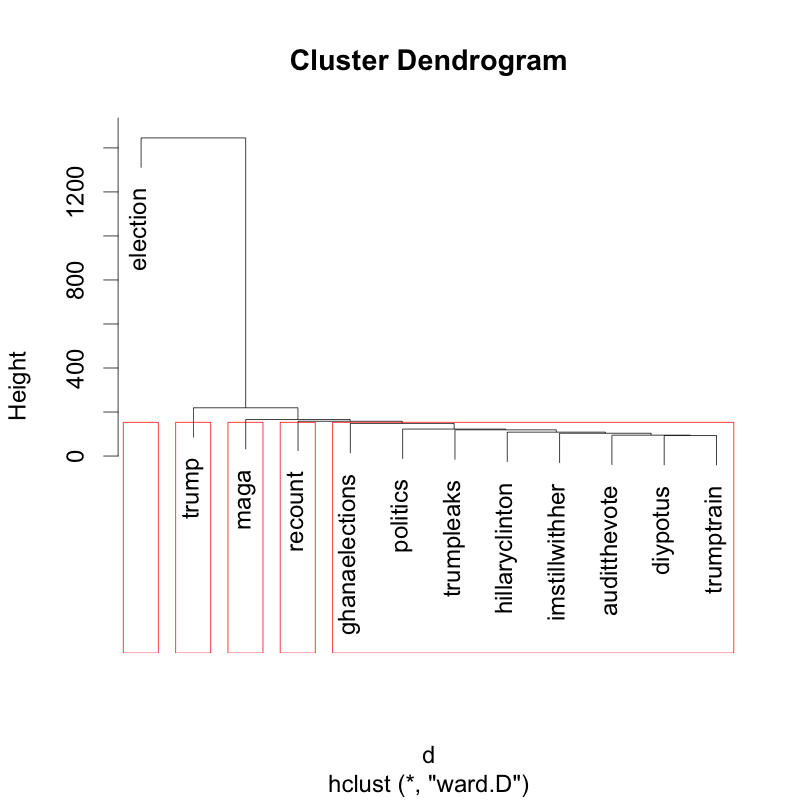
\includegraphics[width = \textwidth]{cluster-election2016}
\caption{A hierarchical cluster of hashtags used with the Election2016 hashtag.}
\label{election2016 cluster}
\end{minipage}\hfill
\begin{minipage}[b]{.49\textwidth}
    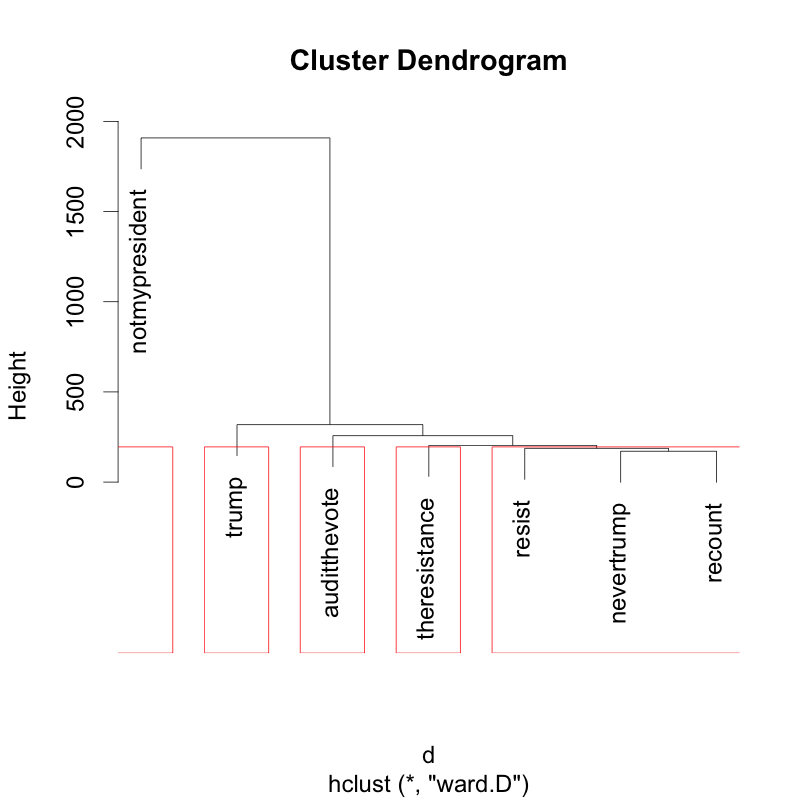
\includegraphics[width = \textwidth]{cluster-notmypresident}
\caption{A hierarchical cluster of hashtags used with the NotMyPresident hashtag.}
\label{notmypresident cluster}
\end{minipage}
\end{figure*}

The \#NotMyPresident hashtag also reflected its projected userbase and deviated
most significantly from the rest of the hashtags. None of the related hashtags
listed in any of the clusters is clearly pro-Trump, and most cite Jill Stein's
proposed audit of the vote or calls to resist Trump's presidency. These hashtags
are entirely expected, as the purpose of the \#NotMyPresident hashtag is in
large part to resist Trump.

\section{Hashtag Sentiments Over Time}
Sentiment analysis was then performed on the tweets in different hashtags in an
attempt to gain insight about what users posting to a certain hashtag thought
about the topics related to that hashtag. The sentiment analysis was performed
with the \verb|syuzhet| package, utilizing the NRC sentiment dictionary by Saif
Mohammad \cite{nrc} to categorize words into ten categories. These ten categories could be
consolidated into ``positive'' or ``negative'' sentiments, which were then
graphed to determine the level of each sentiment present in tweets. Sentiments
are derived from the tweets by tallying the occurrences of each class of word in
each tweet, and tallying the average number of corresponding words in each tweet
over the course of a day. This means that a score of $1$ indicates an average of
one positive word per tweet of either class, and as a result the negative and
positive sentiments in each tweet are viewed separately. 

While this method may seem rather simplistic compared to more sophisticated
classification methods, it was deemed sufficient for the desired analysis. The
\verb|syuzhet| package has been shown to accurately convey the sentiment over
time of literature by classifying individual sentences \cite{jockers}. This
model could easily be extended to the observed hashtags by viewing each tweet as
a sentence in a large corpus of tweets ordered chronologically, making the
\verb|syuzhet| package an appropriate model for classifying sentiment. An
ensemble method employing Naive Bayes, logistic regression, random forests,
neural networks, and support vector machines in conjunction with each other was
tested, but did not achieve strong enough results with sample training data for
further usage.

Despite the reputed negativity of the 2016 presidential election, most hashtags
had a greater number of positive sentiments during collection than negative
sentiments. The only consistent case of a greater number of negative sentiments
than positive ones was with the \#NotMyPresident hashtag over the second
collection window. This is likely indicative of the apparent conservative nature
of the users who post using the collected hashtags. The other unexpected result
of sentiment analysis was the large spike that coincided with an increase in
tweets on a few hashtags. This is likely to indicate a tweet that received a
large number of retweets, but the consistently positive associations and
occurrence across multiple hashtags suggests more review may be necessary to
understand this phenomenon.

\begin{figure*}
\centering
\begin{minipage}[b]{.49\textwidth}
    \includegraphics[width = \textwidth]{set2/sentiment-clinton}
\caption{A sharp spike in positive sentiment on the Clinton hashtag that
  coincides with a sharp increase in tweets.}\label{clinton sentiment}
\end{minipage}\hfill
\begin{minipage}[b]{.49\textwidth}
    \includegraphics[width = \textwidth]{set2/sentiment-maga}
\caption{The MAGA hashtag consistently showed more positive sentiments in tweets
  than negative sentiments.}
\label{maga chart}
\end{minipage}
\end{figure*}

\section{Emoji Analysis}
As an attempt to gain further insight on the sentiments of users posting on the
various hashtags, the emoji in each tweet were stripped out of the tweet text
and placed into a separate field for further analysis. Putting the resulting
string into a term-document matrix and plotting the most-used terms through
\verb|ggplot2| gave further insight as to the sentiments contained in the tweet.

The bar plots indicate that remarkably few users use emoji; perhaps only 1\% of
collected tweets analyzed included any of the top emoji. Furthermore, the two
top emoji in the resulting graphs, ``joy'', and ``+1'', have been suggested to
likely be used for sharp satire \cite{emoji}. The sentiment analysis performed
through even sophisticated classification methods would be unlikely to pick up
on the nuances induced by this, which may suggest inherent difficulties in
sentiment analysis. The frequency with which these two emoji appear in the
collected tweets indicate that many of the positive sentiments found in the
different hashtags may in fact source from satire or other humor. This would go
to explain the unexpected level of positive sentiment, but would not provide a
clear solution for how to properly classify those sentiments.

\begin{figure*}
\centering
\begin{minipage}[b]{.49\textwidth}
    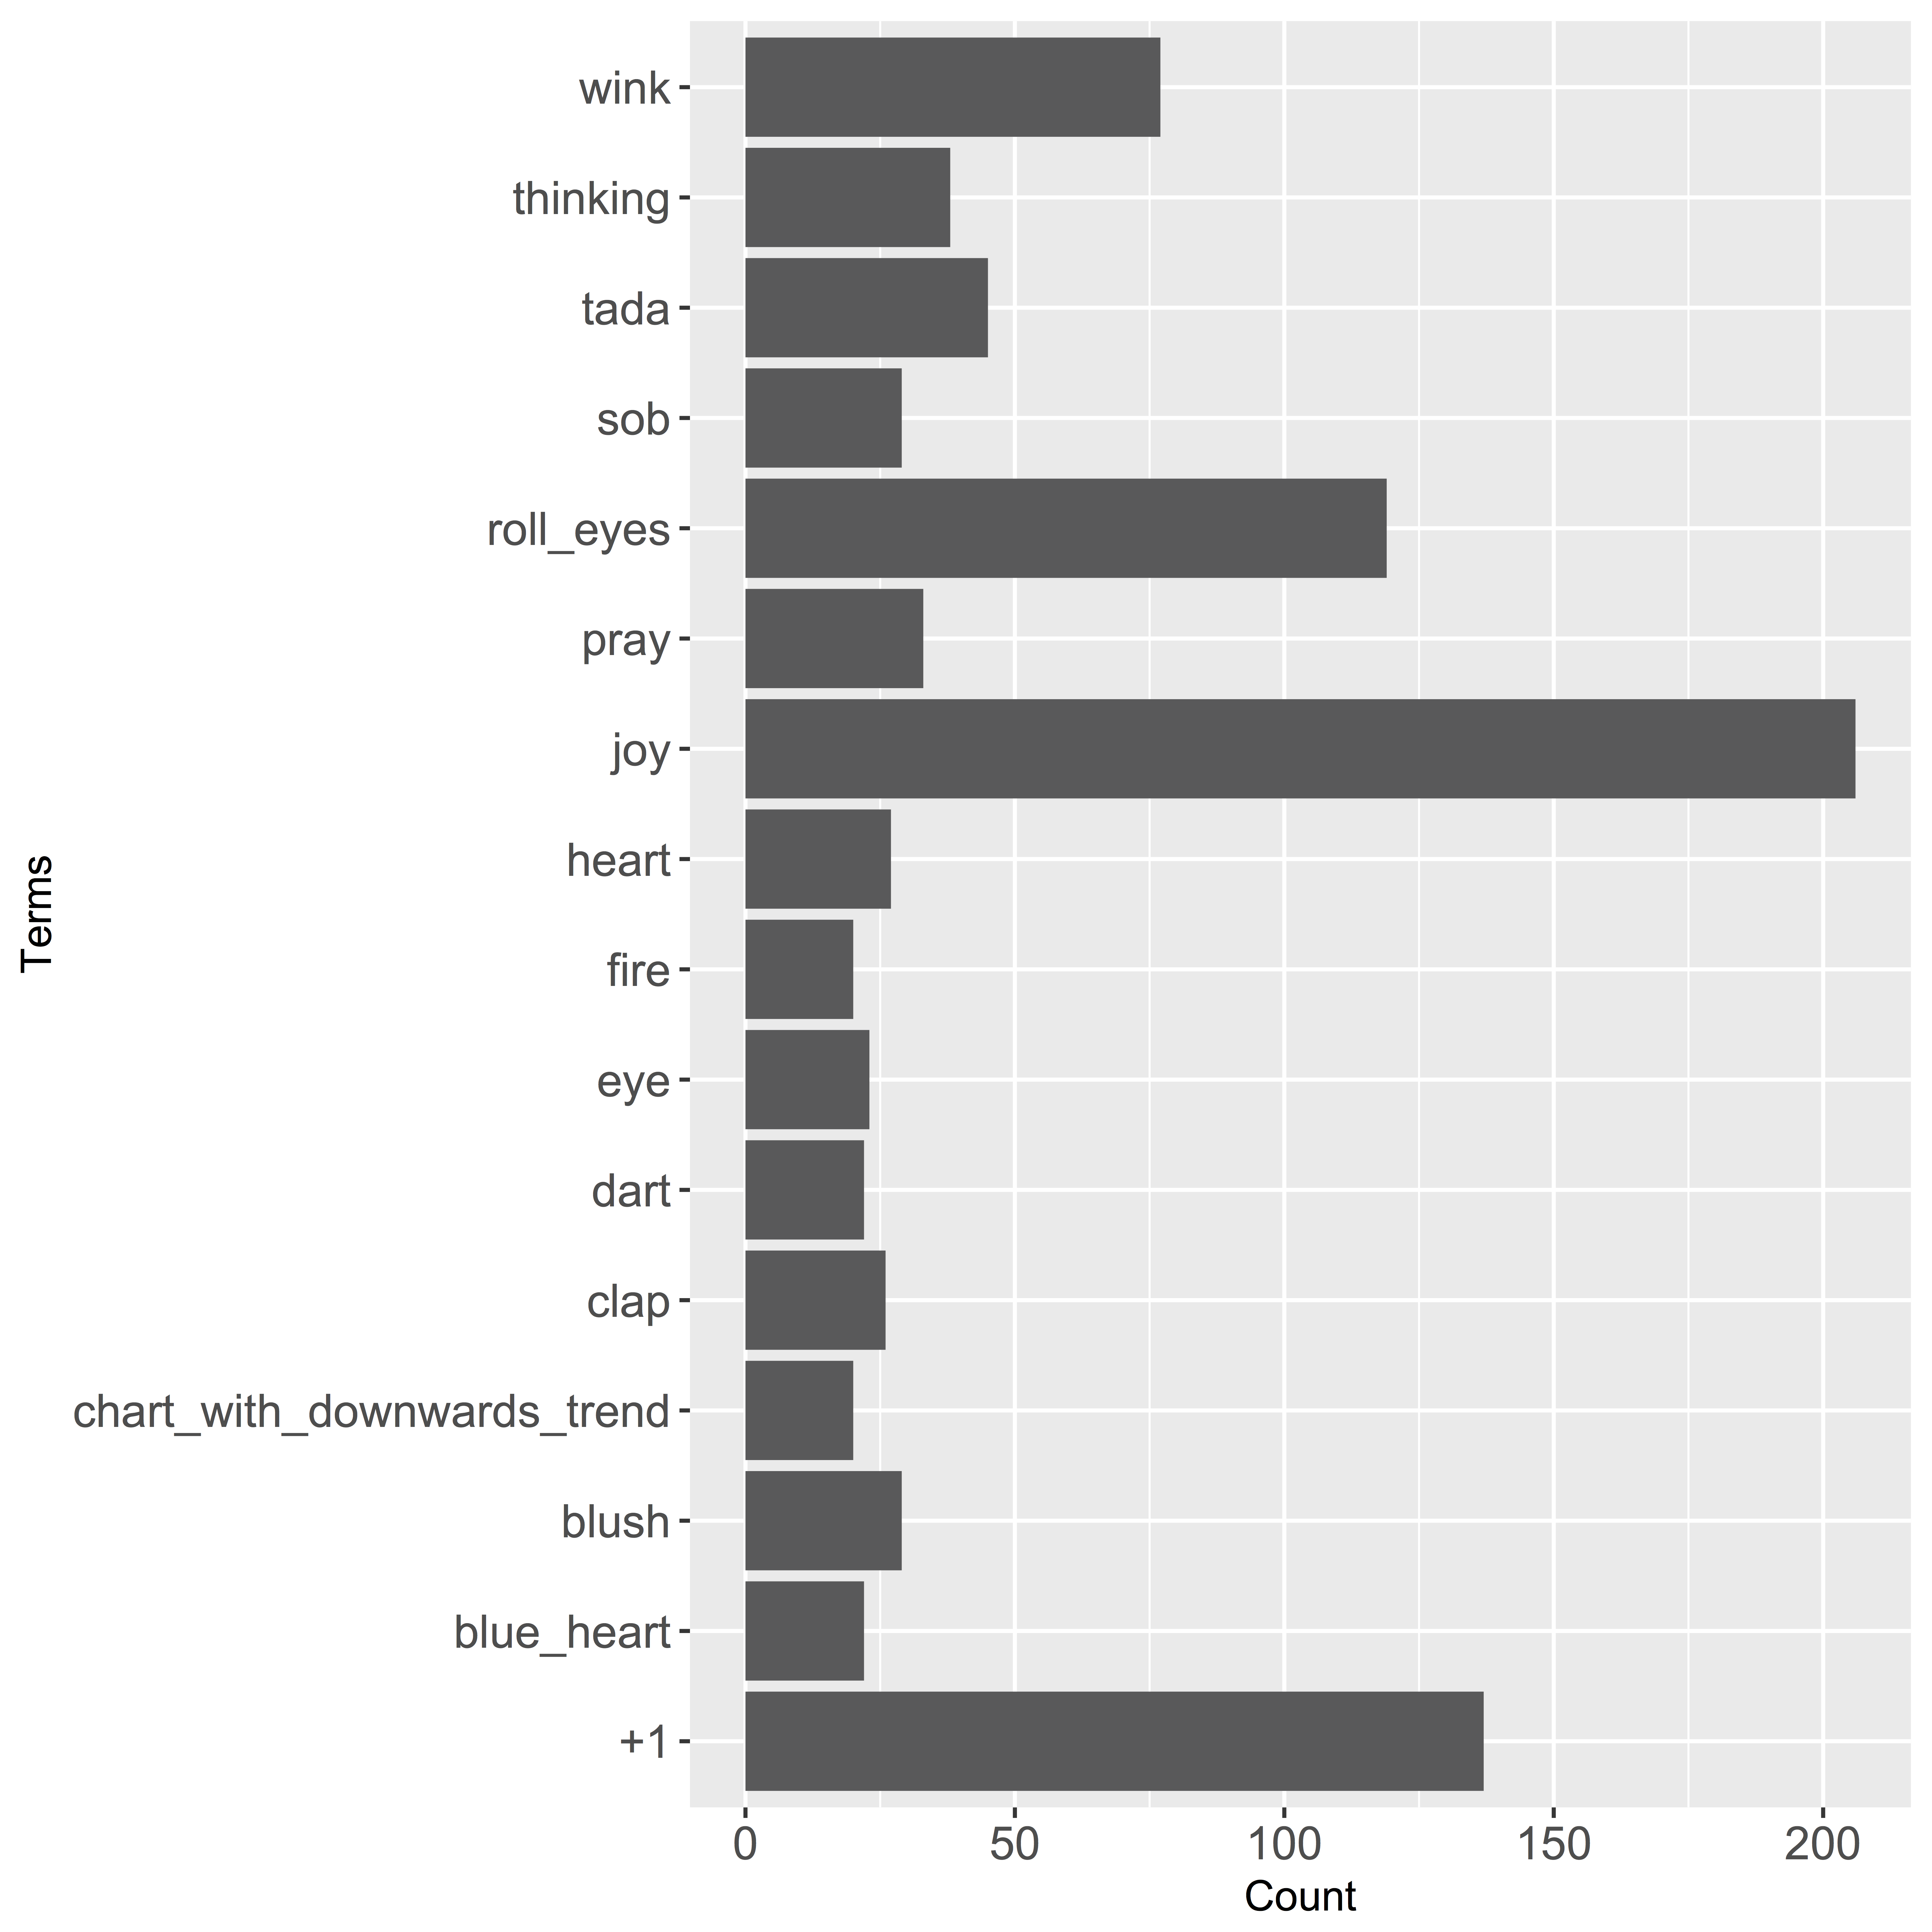
\includegraphics[width = \textwidth]{emoji-election2016}
\caption{The top emoji used in the tweets collected in Election2016 during the
  first window.}
\label{election2016 emoji}
\end{minipage}\hfill
\begin{minipage}[b]{.49\textwidth}
    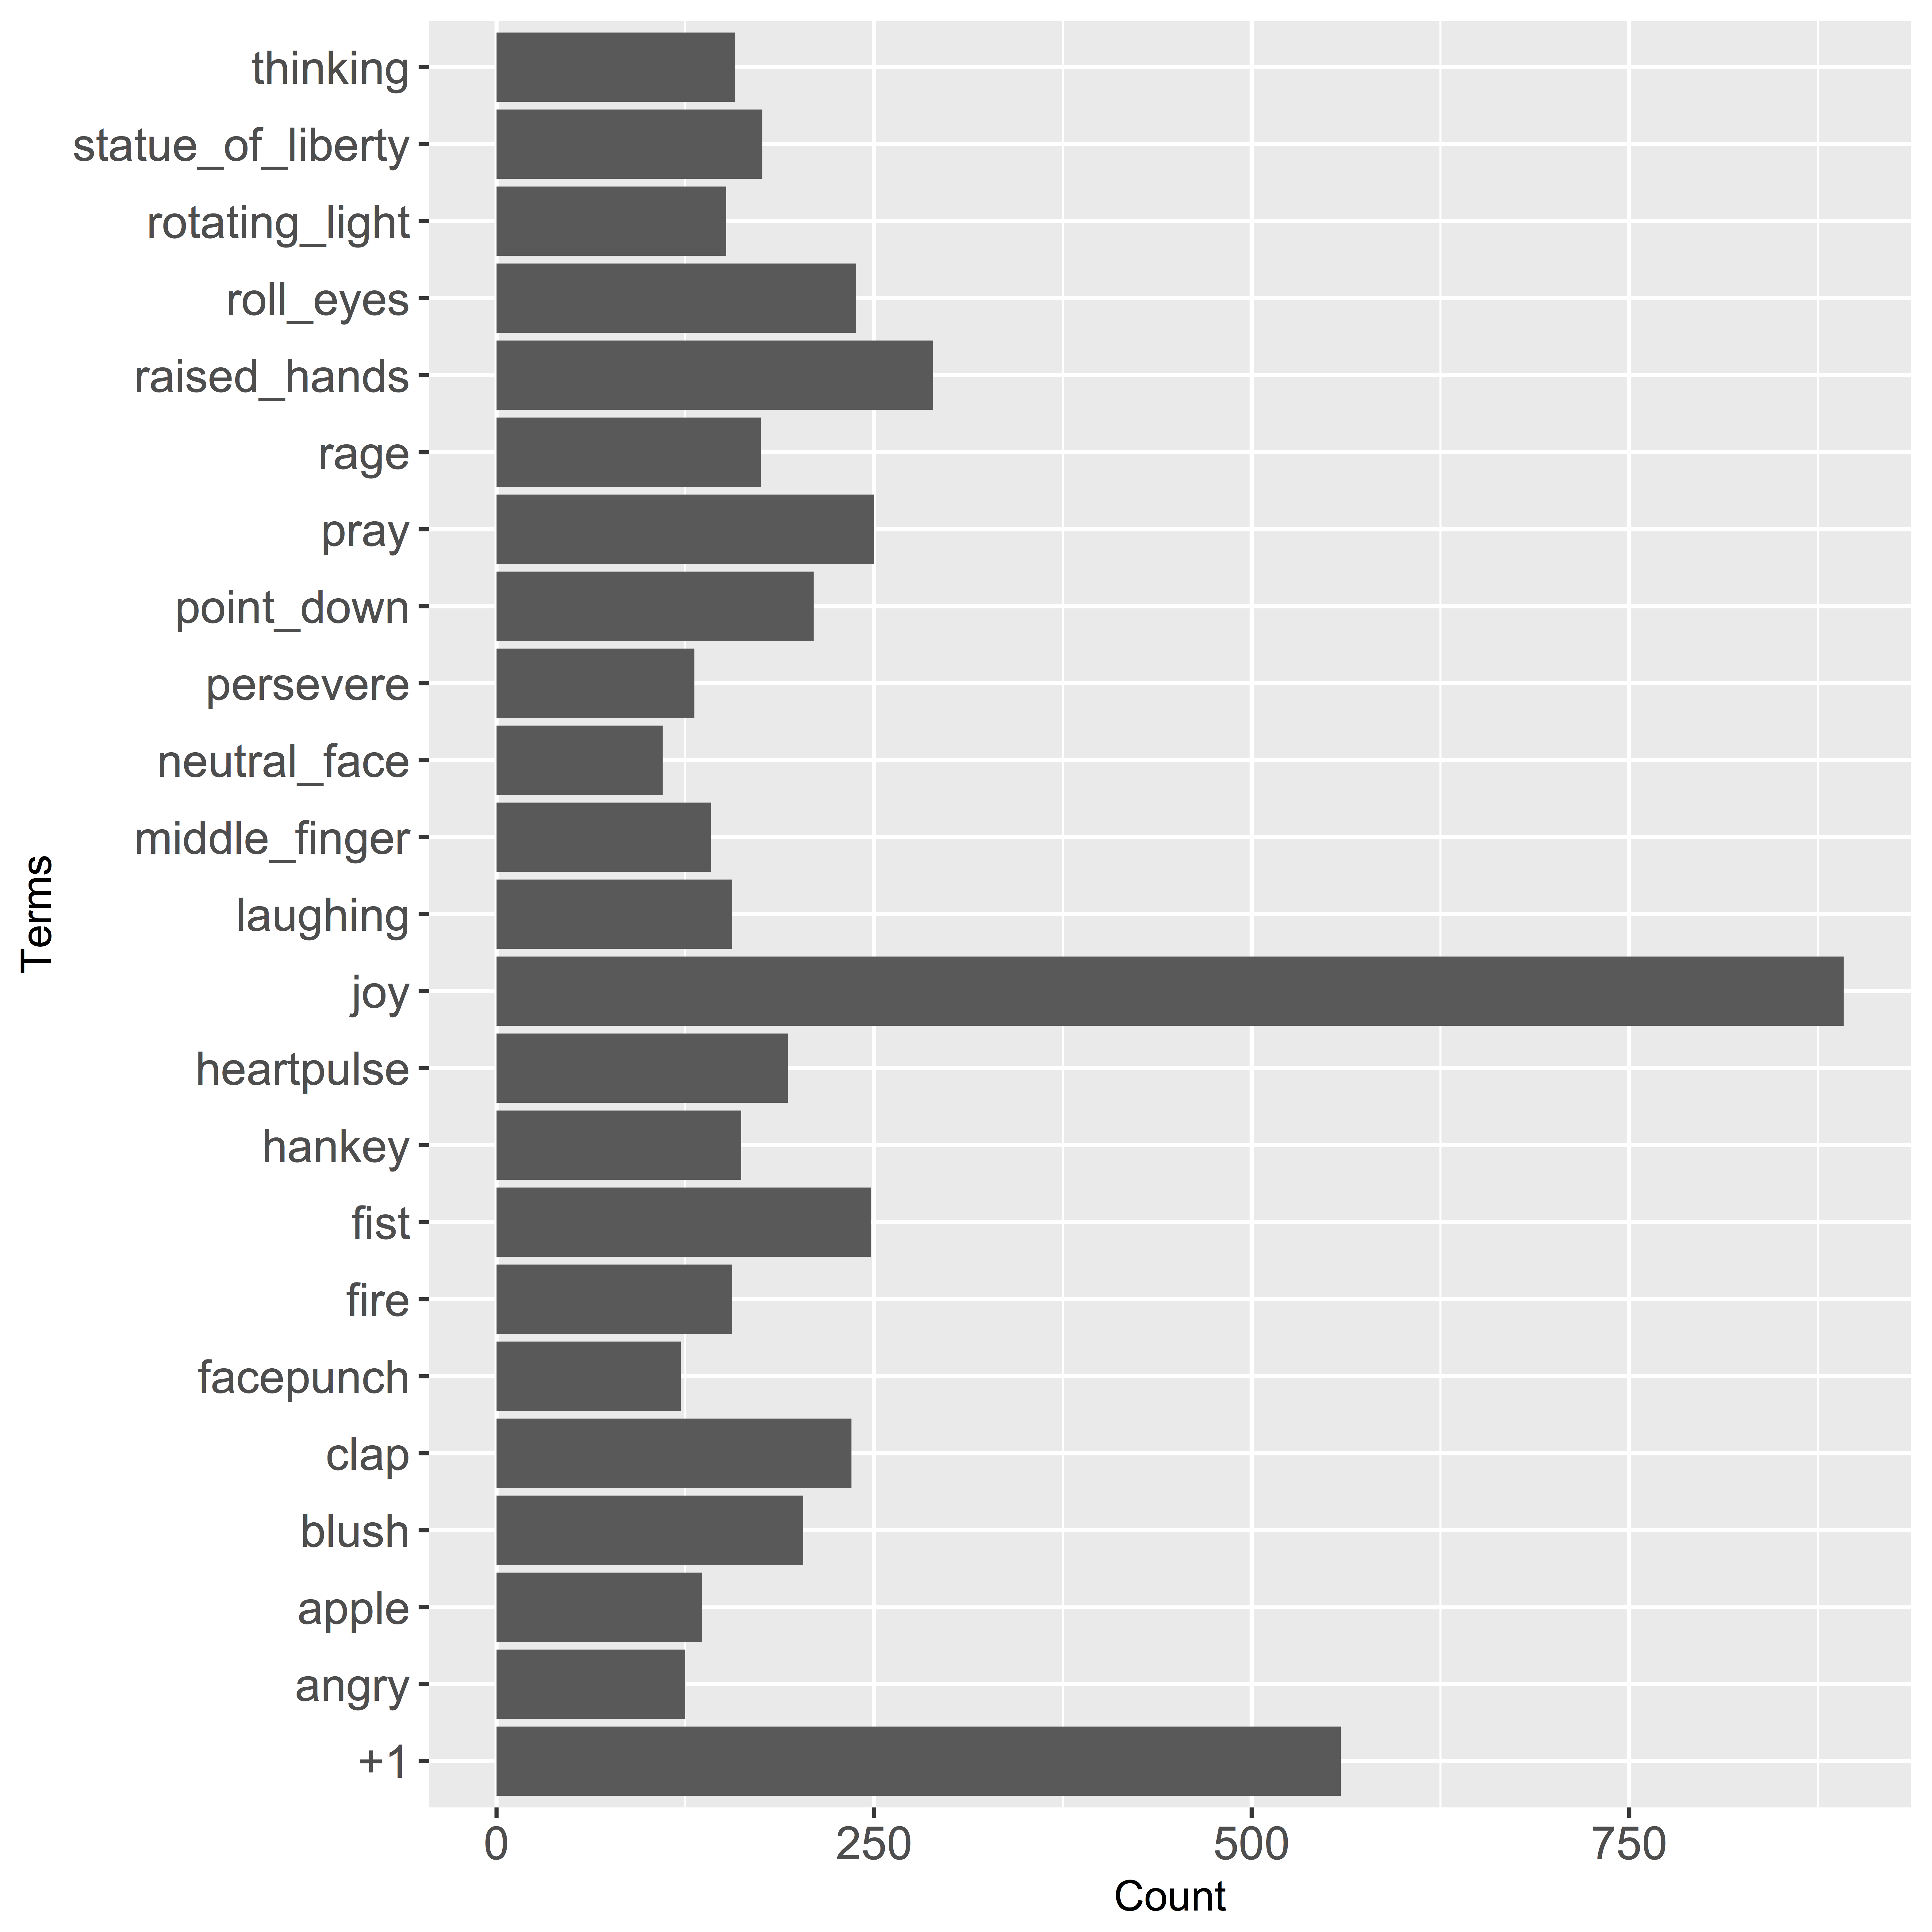
\includegraphics[width = \textwidth]{emoji-notmypresident}
\caption{The top emoji used in the tweets collectedin NotMyPresident during the first window.}
\label{notmypresident emoji}
\end{minipage}
\end{figure*}

%\begin{figure}[!t]
%  \tbl{The overall process used in testing the classifiers.}{
%    \includegraphics[width = \textwidth]{process}}
%\end{figure}

%\begin{table}[!t]
%  \tbl{Confusion matrix generated by the decision tree with all attributes and
%    no re-sampling.}{
%    \includegraphics[width = \textwidth]{dt-aa-nos}}
%\end{table}

\section{Conclusions}
Analyzing the hashtags separately revealed that Trump has a wide base of support
on Twitter, and furthermore that they are actively engaged and generally
positive about political events that have happened in the weeks following the
election. It would also appear that the majority of political conversation that
occurs on Twitter deals with Trump to some degree, which is to be expected due
to his recent upset victory for what many consider to be the most important
political office in the United States.

The work laid out in this paper can stand to benefit from a number of
improvements in methodology to better determine the American political
atmosphere, however. In particular, a more sophisticated system that watches
tweet trends to determine what hashtags to collect would provide better samples
of tweets that capture a larger number and more diverse set of tweets. This
could be easily accomplished by watching the secondary hashtags that emerge in
the collected hashtags and begin collection on the most popular secondary
hashtags while pruning hashtags that do not seem to offer any insights. Stream
mining techniques could also be applied to this model to gather data on the
hashtags without the need to store immense amounts of data, and could also offer
online analysis of the hashtags. 

With better user samples, hypothetically geographic location could also be
considered for each tweet to construct a colored map of the United States. This
could then be compared to the electoral map representing the popular vote in the
2016 presidential election to gain further insights about which areas these
users come from and to gain further insights about the political atmosphere in
the United States. This would most importantly require a better sample of
tweets, however, to properly represent the relative makeup of the United States.
Mapping the collected tweets was deemed unnecessary due to their significant
conservative makeup, which would almost certainly skew the map results.

Emoji analysis could also provide greater feedback as to what users are thinking
if employed correctly due to the relatively specific emotions they express.
However, the usage of emoji is wildly inconsistent, with different users using
emoji in different ways, and the emoji changing meanings in different contexts.
These factors would need to be accounted for if the results were to be accurate.

\bibliographystyle{acm}
\bibliography{references}
%\printbibliography
% \section{References}
% S. Moro, P. Cortez and P. Rita. A Data-Driven Approach to Predict the Success
% of Bank Telemarketing. Decision Support Systems, Elsevier, 62:22-31, June 2014

\section{Appendix}
\newpage

% Frequencies; set 1
\begin{figure}[!t]
  \tbl{Election2016 trend histogram for the first window of collected tweets.}{
    \includegraphics[width = .60\textwidth]{set1/freq-election2016}}
\end{figure}

\begin{figure}[!t]
  \tbl{ElectionNight trend histogram for the first window of collected tweets.}{
    \includegraphics[width = .60\textwidth]{set1/freq-electionnight}}
\end{figure}

\begin{figure}[!t]
  \tbl{NotMyPresident trend histogram for the first window of collected tweets.}{
    \includegraphics[width = .60\textwidth]{set1/freq-notmypresident}}
\end{figure}

%Frequencies; set 2
\begin{figure}[!t]
  \tbl{AmericaFirst trend histogram for the second window of collected tweets.}{
    \includegraphics[width = .60\textwidth]{set2/freq-americafirst}}
\end{figure}

\begin{figure}[!t]
  \tbl{Clinton trend histogram for the second window of collected tweets.}{
    \includegraphics[width = .60\textwidth]{set2/freq-clinton}}
\end{figure}

\begin{figure}[!t]
  \tbl{DrainTheSwamp trend histogram for the second window of collected tweets.}{
    \includegraphics[width = .60\textwidth]{set2/freq-draintheswamp}}
\end{figure}

\begin{figure}[!t]
  \tbl{Election2016 trend histogram for the second window of collected tweets.}{
    \includegraphics[width = .60\textwidth]{set2/freq-election2016}}
\end{figure}

\begin{figure}[!t]
  \tbl{ElectionNight trend histogram for the second window of collected tweets.}{
    \includegraphics[width = .60\textwidth]{set2/freq-electionnight}}
\end{figure}

\begin{figure}[!t]
  \tbl{MAGA trend histogram for the second window of collected tweets.}{
    \includegraphics[width = .60\textwidth]{set2/freq-maga}}
\end{figure}

\begin{figure}[!t]
  \tbl{MakeAmericaGreatAgain trend histogram for the second window of collected tweets.}{
    \includegraphics[width = .60\textwidth]{set2/freq-makeamericagreatagain}}
\end{figure}

\begin{figure}[!t]
  \tbl{NotMyPresident trend histogram for the second window of collected tweets.}{
    \includegraphics[width = .60\textwidth]{set2/freq-notmypresident}}
\end{figure}

\begin{figure}[!t]
  \tbl{Trump trend histogram for the second window of collected tweets.}{
    \includegraphics[width = .60\textwidth]{set2/freq-trump}}
\end{figure}

% Wordclouds
\begin{figure}[!t]
  \tbl{AmericaFirst wordcloud compiled from user biographies.}{
    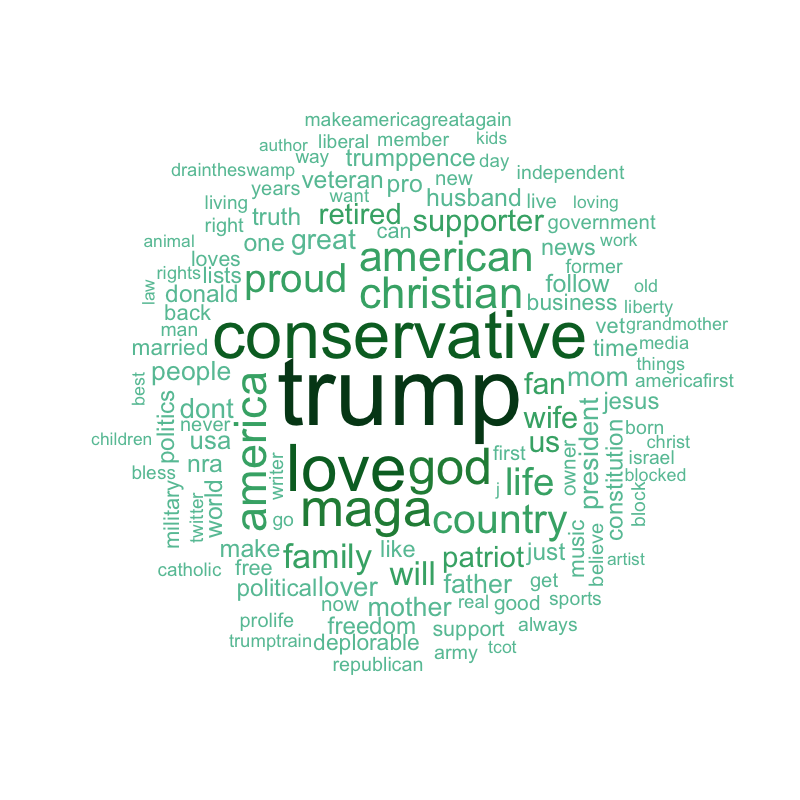
\includegraphics[width = .60\textwidth]{cloud-americafirst}}
\end{figure}

\begin{figure}[!t]
  \tbl{Clinton wordcloud compiled from user biographies.}{
    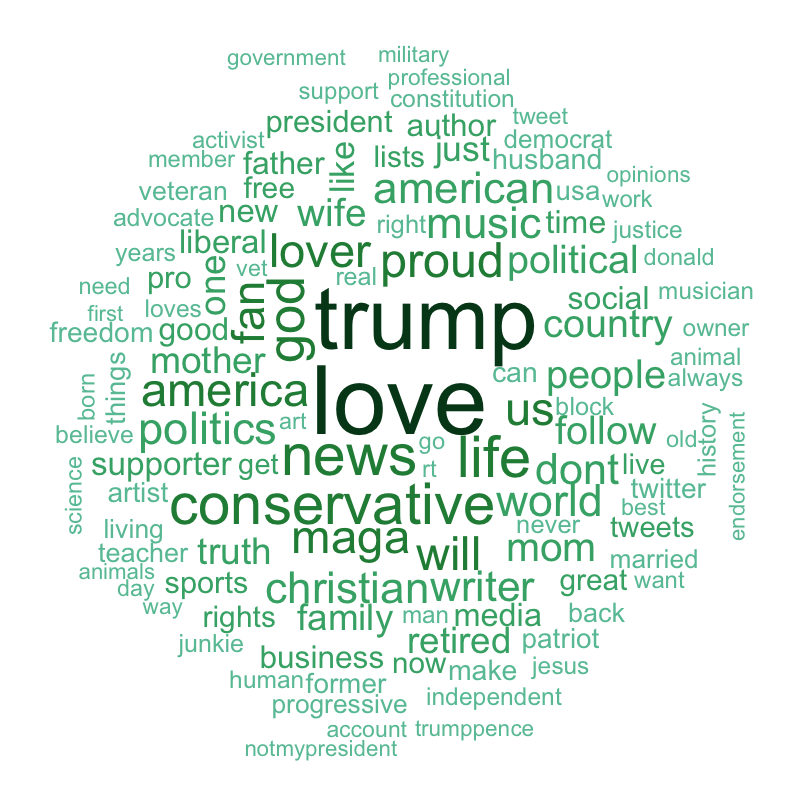
\includegraphics[width = .60\textwidth]{cloud-clinton}}
\end{figure}

\begin{figure}[!t]
  \tbl{DrainTheSwamp wordcloud compiled from user biographies.}{
    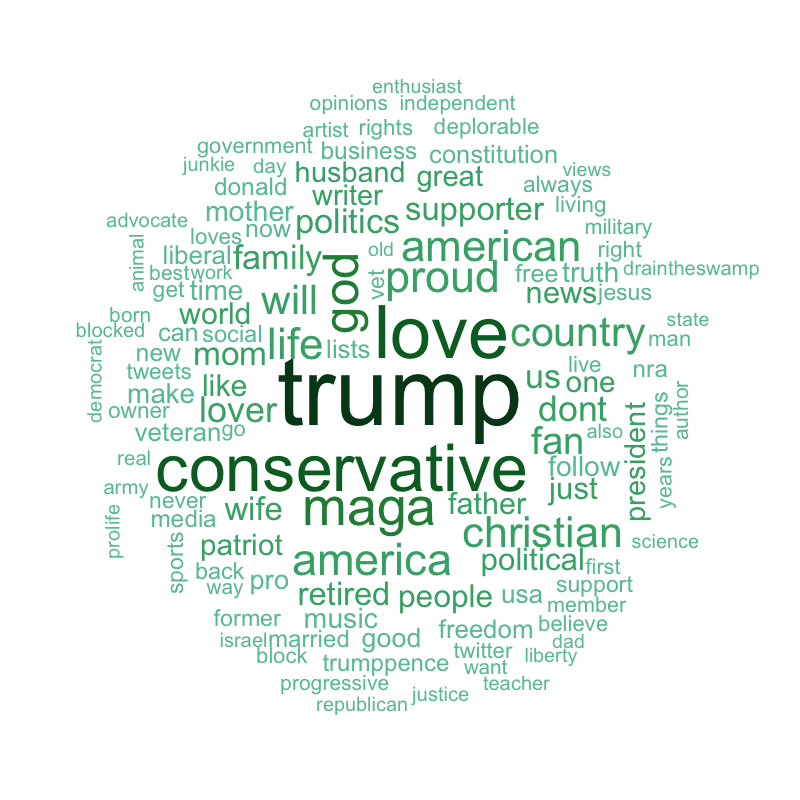
\includegraphics[width = .60\textwidth]{cloud-draintheswamp}}
\end{figure}

\begin{figure}[!t]
  \tbl{Election2016 wordcloud compiled from user biographies.}{
    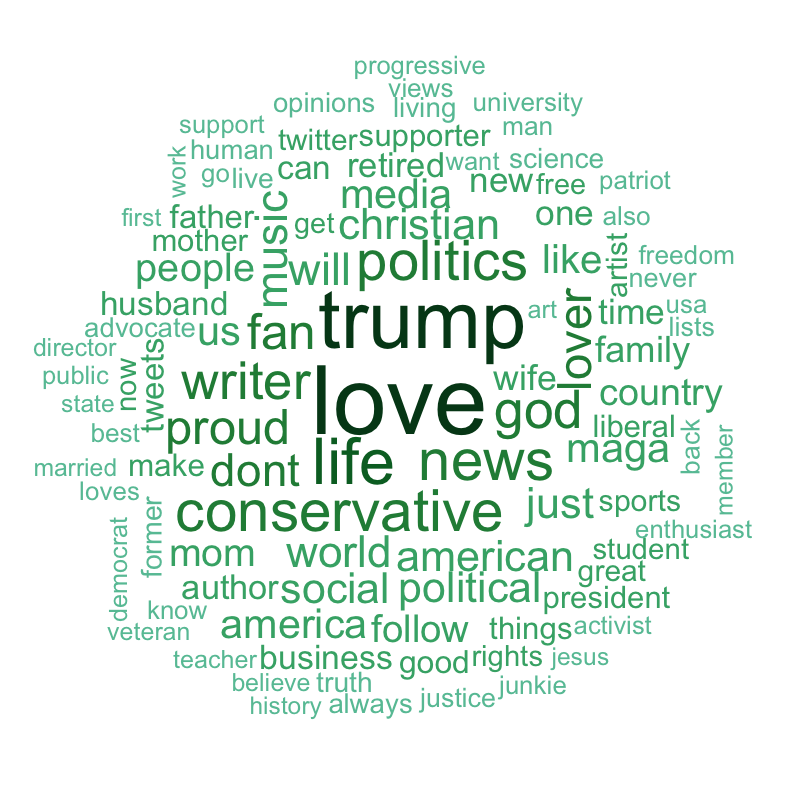
\includegraphics[width = .60\textwidth]{cloud-election2016}}
\end{figure}

\begin{figure}[!t]
  \tbl{ElectionNight wordcloud compiled from user biographies.}{
    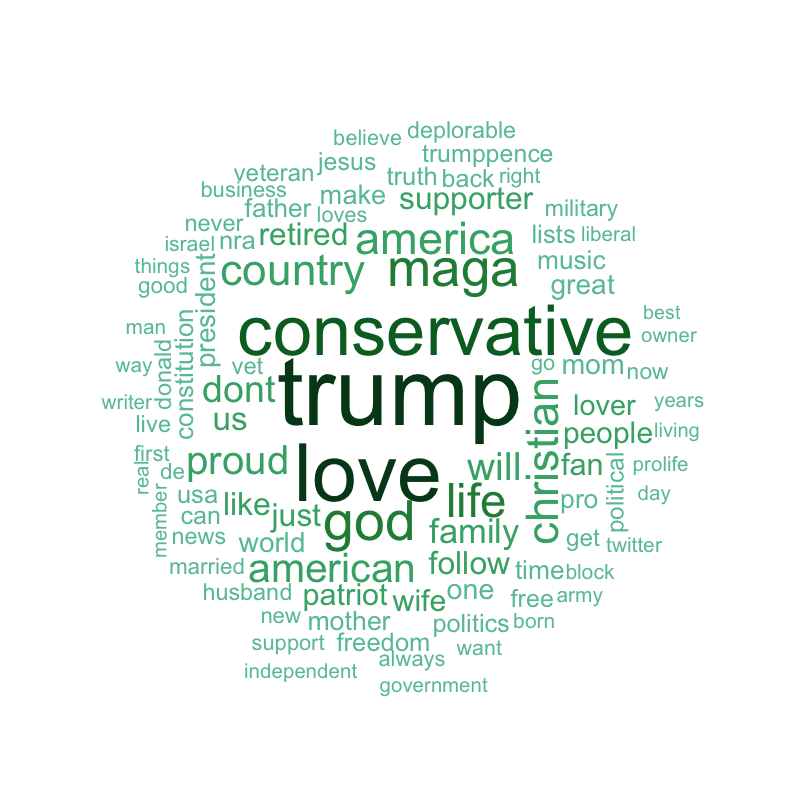
\includegraphics[width = .60\textwidth]{cloud-electionnight}}
\end{figure}

\begin{figure}[!t]
  \tbl{MAGA wordcloud compiled from user biographies.}{
    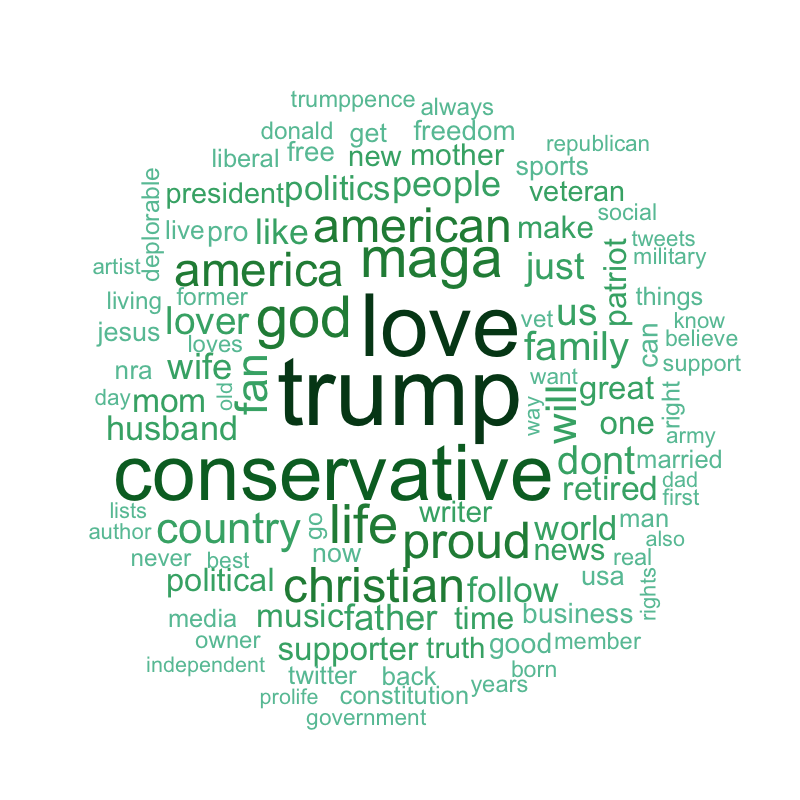
\includegraphics[width = .60\textwidth]{cloud-maga}}
\end{figure}

\begin{figure}[!t]
  \tbl{MakeAmericaGreatAgain wordcloud compiled from user biographies.}{
    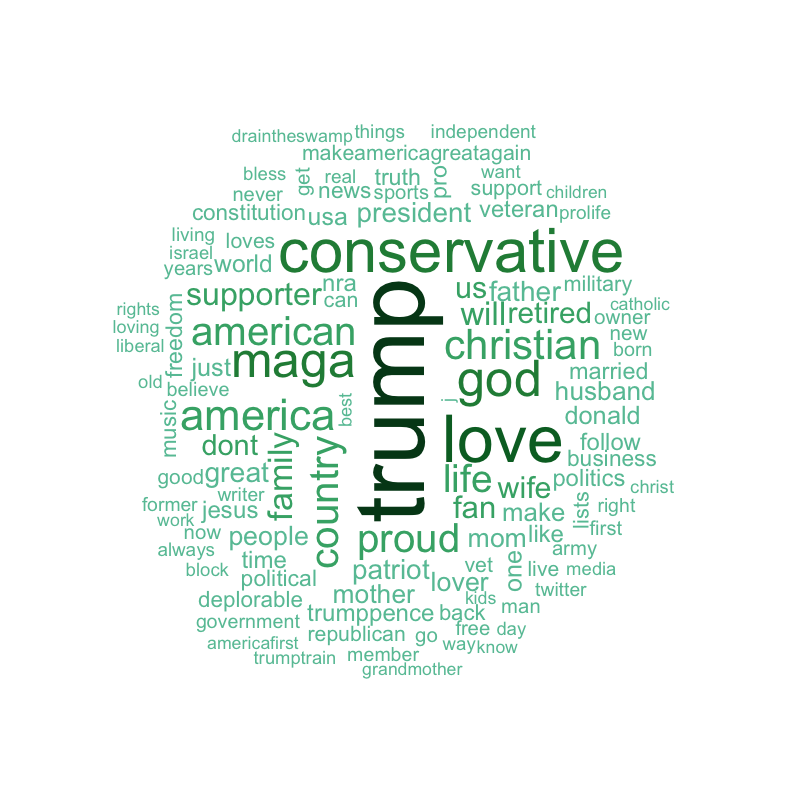
\includegraphics[width = .60\textwidth]{cloud-makeamericagreatagain}}
\end{figure}

\begin{figure}[!t]
  \tbl{NotMyPresident wordcloud compiled from user biographies.}{
    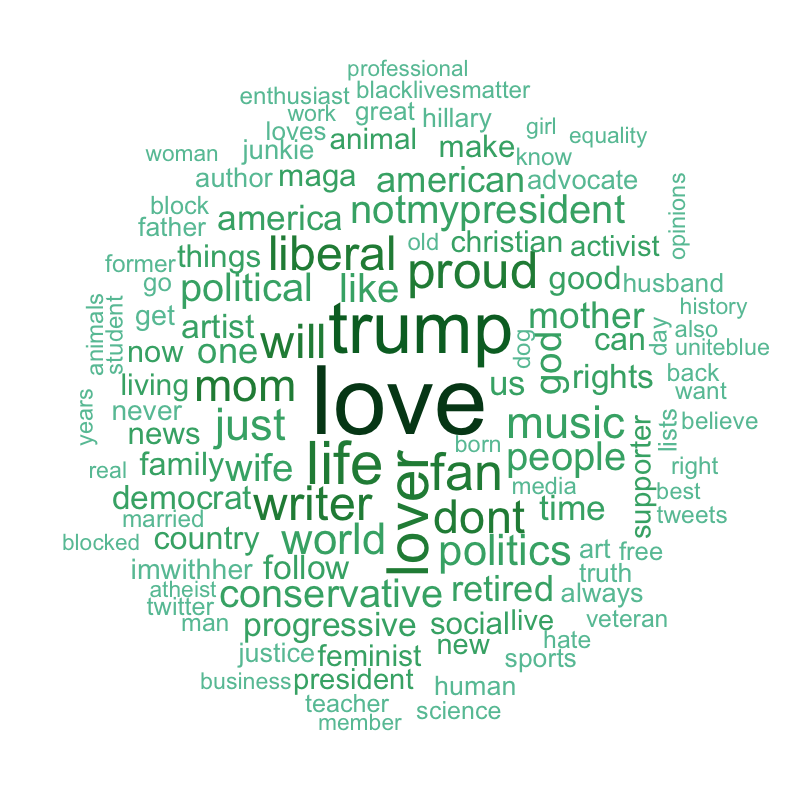
\includegraphics[width = .60\textwidth]{cloud-notmypresident}}
\end{figure}

\begin{figure}[!t]
  \tbl{Trump wordcloud compiled from user biographies.}{
    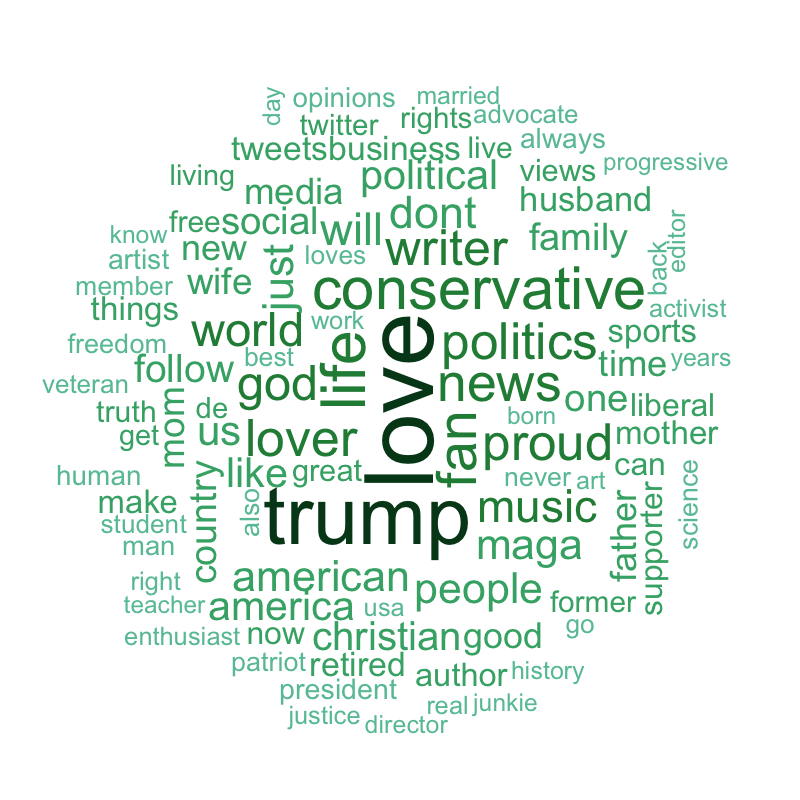
\includegraphics[width = .60\textwidth]{cloud-trump}}
\end{figure}

% Hashtag clusters 
\begin{figure}[!t]
  \tbl{AmericaFirst hierarchical cluster compiled from hashtags in tweet.}{
    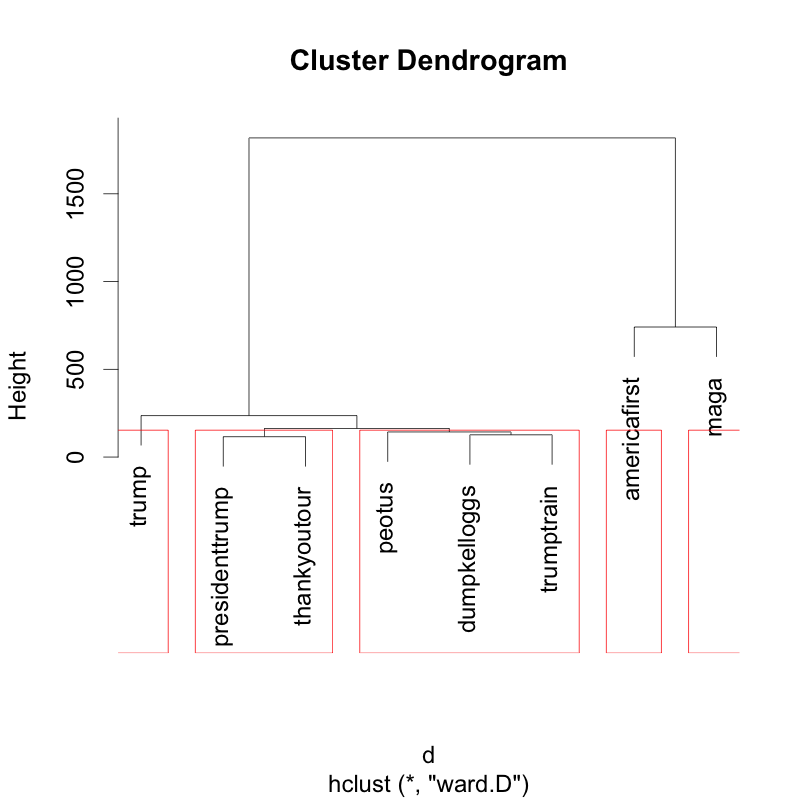
\includegraphics[width = .60\textwidth]{cluster-americafirst}}
\end{figure}

\begin{figure}[!t]
  \tbl{Clinton hierarchical cluster compiled from hashtags in tweet.}{
    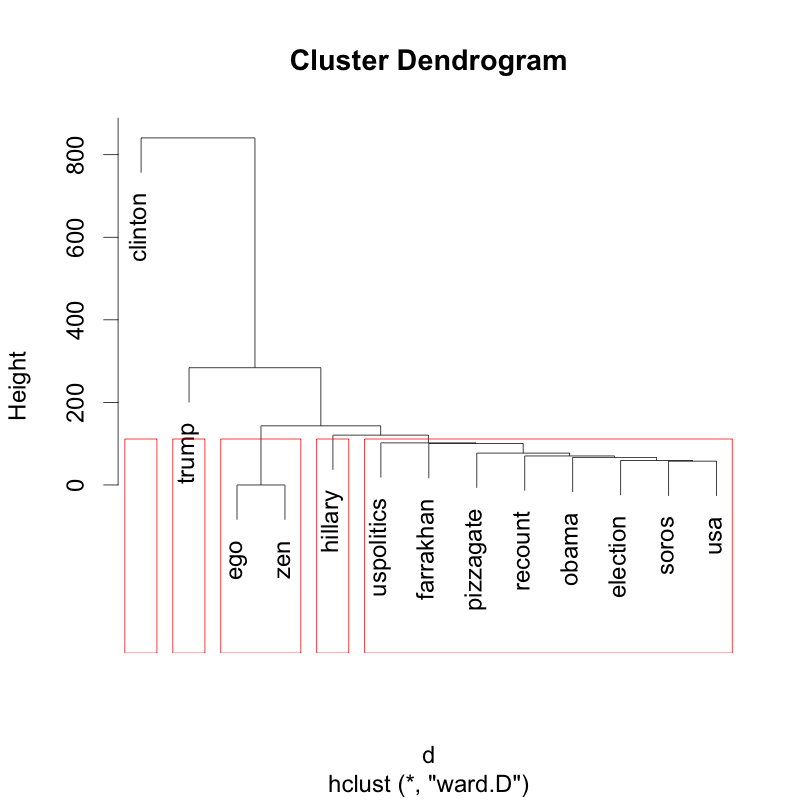
\includegraphics[width = .60\textwidth]{cluster-clinton}}
\end{figure}

\begin{figure}[!t]
  \tbl{DrainTheSwamp hierarchical cluster compiled from hashtags in tweet.}{
    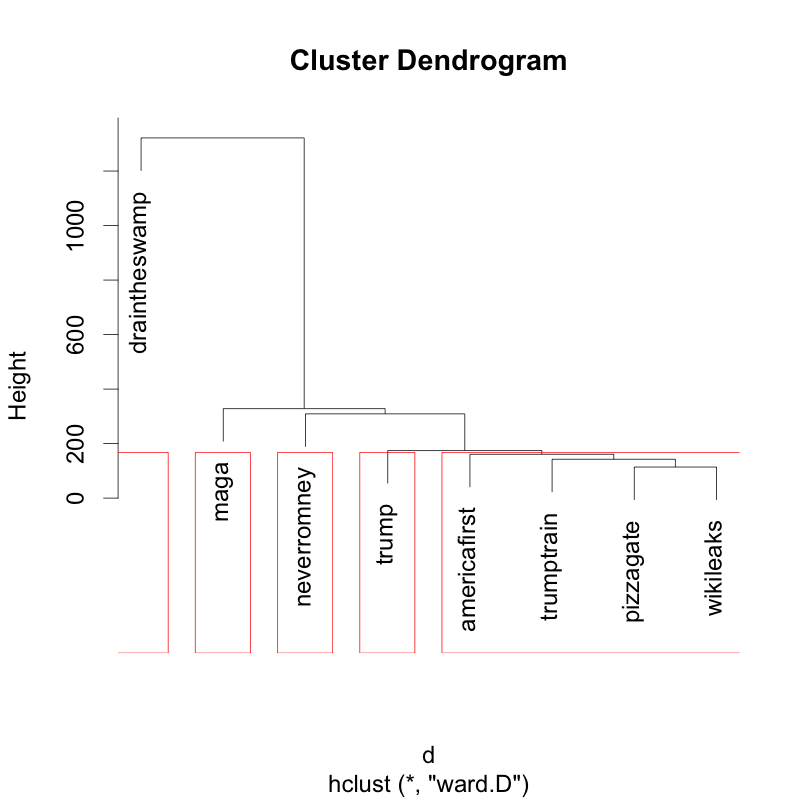
\includegraphics[width = .60\textwidth]{cluster-draintheswamp}}
\end{figure}

\begin{figure}[!t]
  \tbl{Election2016 hierarchical cluster compiled from hashtags in tweet.}{
    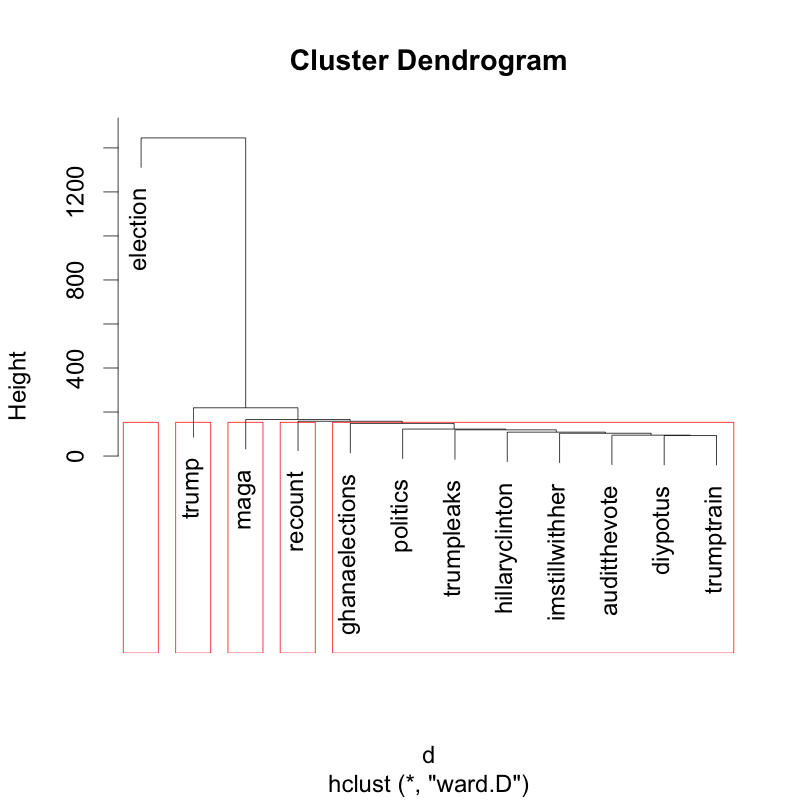
\includegraphics[width = .60\textwidth]{cluster-election2016}}
\end{figure}

\begin{figure}[!t]
  \tbl{ElectionNight hierarchical cluster compiled from hashtags in tweet.}{
    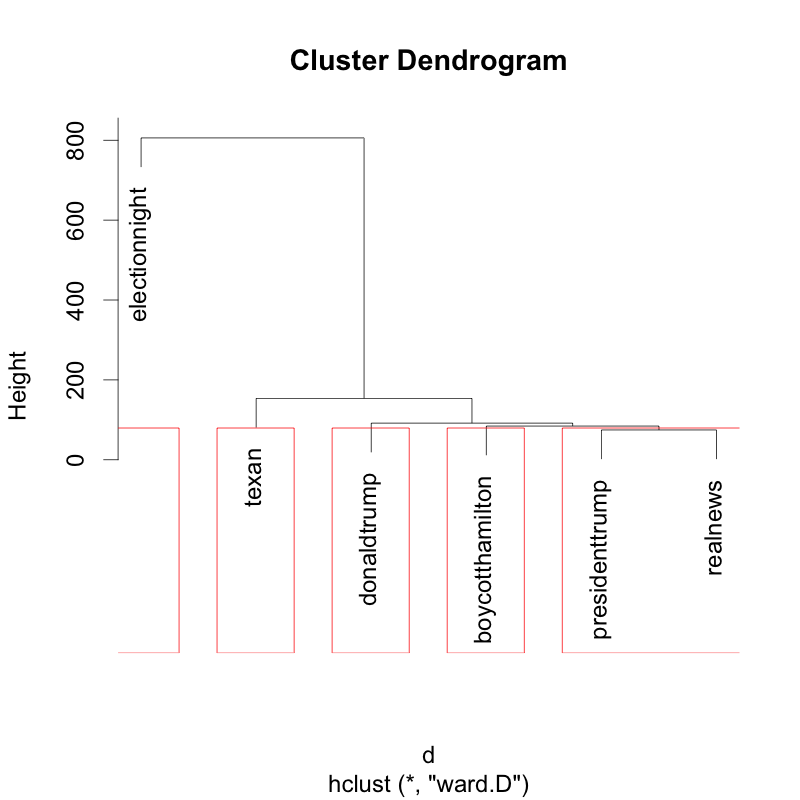
\includegraphics[width = .60\textwidth]{cluster-electionnight}}
\end{figure}

\begin{figure}[!t]
  \tbl{MAGA hierarchical cluster compiled from hashtags in tweet.}{
    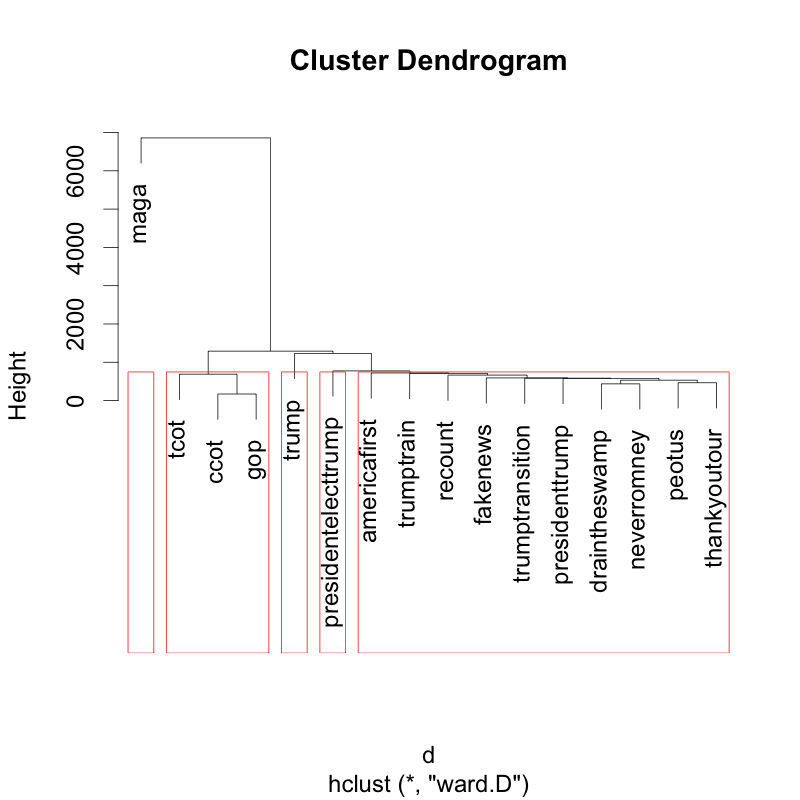
\includegraphics[width = .60\textwidth]{cluster-maga}}
\end{figure}

\begin{figure}[!t]
  \tbl{MakeAmericaGreatAgain hierarchical cluster compiled from hashtags in tweet.}{
    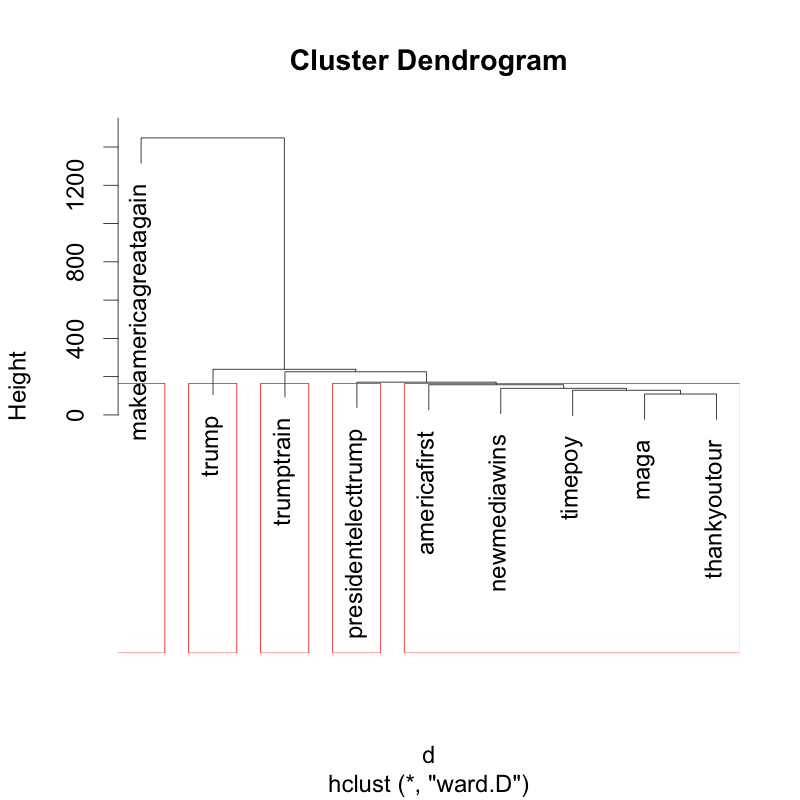
\includegraphics[width = .60\textwidth]{cluster-makeamericagreatagain}}
\end{figure}

\begin{figure}[!t]
  \tbl{NotMyPresident hierarchical cluster compiled from hashtags in tweet.}{
    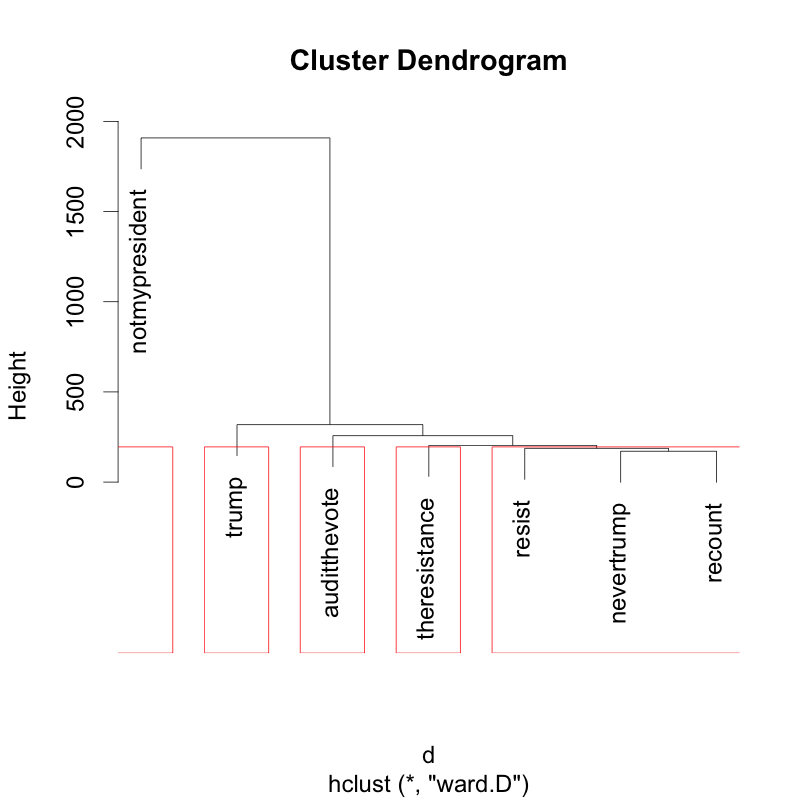
\includegraphics[width = .60\textwidth]{cluster-notmypresident}}
\end{figure}

\begin{figure}[!t]
  \tbl{Trump hierarchical cluster compiled from hashtags in tweet.}{
    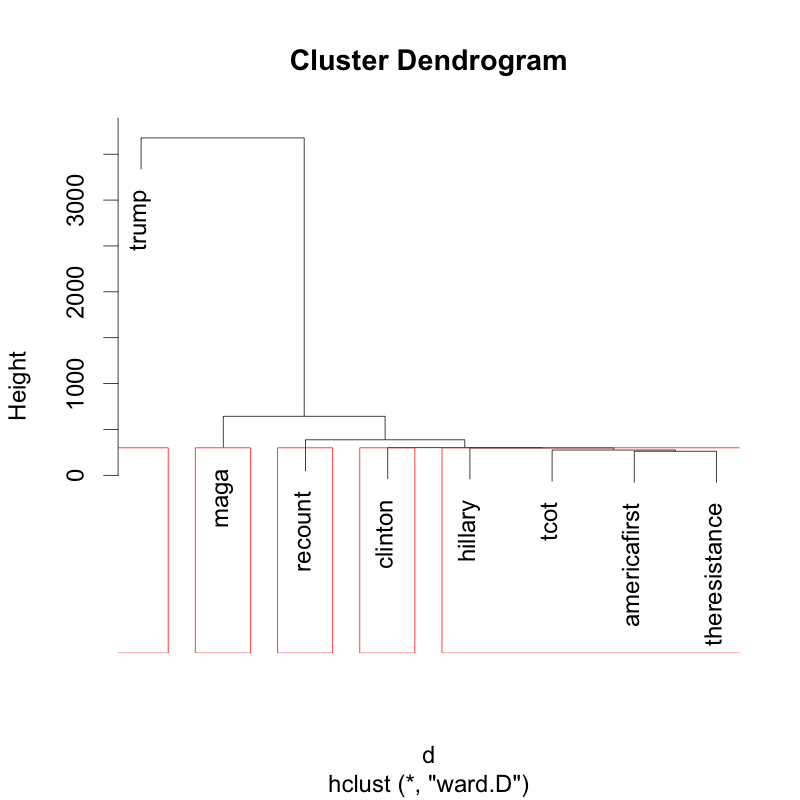
\includegraphics[width = .60\textwidth]{cluster-trump}}
\end{figure}

% Sentiment; set 1
\begin{figure}[!t]
  \tbl{Election2016 sentiment plot for first window of collected tweets.}{
    \includegraphics[width = .60\textwidth]{set1/sentiment-election2016}}
\end{figure}

\begin{figure}[!t]
  \tbl{ElectionNight sentiment plot for first window of collected tweets.}{
    \includegraphics[width = .60\textwidth]{set1/sentiment-electionnight}}
\end{figure}

\begin{figure}[!t]
  \tbl{NotMyPresident sentiment plot for first window of collected tweets.}{
    \includegraphics[width = .60\textwidth]{set1/sentiment-notmypresident}}
\end{figure}

%Sentiment; set 2
\begin{figure}[!t]
  \tbl{AmericaFirst sentiment plot for second window of collected tweets.}{
    \includegraphics[width = .60\textwidth]{set2/sentiment-americafirst}}
\end{figure}

\begin{figure}[!t]
  \tbl{Clinton sentiment plot for second window of collected tweets.}{
    \includegraphics[width = .60\textwidth]{set2/sentiment-clinton}}
\end{figure}

\begin{figure}[!t]
  \tbl{DrainTheSwamp sentiment plot for second window of collected tweets.}{
    \includegraphics[width = .60\textwidth]{set2/sentiment-draintheswamp}}
\end{figure}

\begin{figure}[!t]
  \tbl{Election2016 sentiment plot for second window of collected tweets.}{
    \includegraphics[width = .60\textwidth]{set2/sentiment-election2016}}
\end{figure}

\begin{figure}[!t]
  \tbl{ElectionNight sentiment plot for second window of collected tweets.}{
    \includegraphics[width = .60\textwidth]{set2/sentiment-electionnight}}
\end{figure}

\begin{figure}[!t]
  \tbl{MAGA sentiment plot for second window of collected tweets.}{
    \includegraphics[width = .60\textwidth]{set2/sentiment-maga}}
\end{figure}

\begin{figure}[!t]
  \tbl{MakeAmericaGreatAgain sentiment plot for second window of collected tweets.}{
    \includegraphics[width = .60\textwidth]{set2/sentiment-makeamericagreatagain}}
\end{figure}

\begin{figure}[!t]
  \tbl{NotMyPresident sentiment plot for second window of collected tweets.}{
    \includegraphics[width = .60\textwidth]{set2/sentiment-notmypresident}}
\end{figure}

\begin{figure}[!t]
  \tbl{Trump sentiment plot for second window of collected tweets.}{
    \includegraphics[width = .60\textwidth]{set2/sentiment-trump}}
\end{figure}

\begin{figure}[!t]
  \tbl{Emoji frequencies for Election2016 tweets collected in the first window.}{
    \includegraphics[width = .60\textwidth]{emoji-election2016}}
\end{figure}

\begin{figure}[!t]
  \tbl{Emoji frequencies for NotMyPresident tweets collected in the first window.}{
    \includegraphics[width = .60\textwidth]{emoji-notmypresident}}
\end{figure}

\begin{figure}[!t]
  \tbl{stream.js -- Pulled data from Twitter.}{}
    \begin{lstlisting}
const fs = require('fs');
const Twit = require("twit");
const client = new Twit({});
let data;
let filename = "data";
let filepath = __dirname + "/" + filename;
let exists = true;
let lines = 0;
let num = -1;
function createStream() {
    data = fs.createWriteStream(filename + "-" + num + ".json", {
        flags: "w",
        encoding: "utf8",
        mode: 0744
    });
    data.on("error", (error) => {
        console.log("ERROR: " + error);
        num++;
        createStream();
    });
    data.write("{ \"json\": [\n");
}
function listenForData() {
    const stream = client.stream('statuses/filter', { track: tags });

    stream.on('tweet', function (tweet) {
        text = JSON.stringify(tweet);
        if(lines > 50000) {
            data.write("\n]}");
            data.end();
            num++;
            createStream();
            lines = 0;
        } else if(lines > 0) {
            data.write(",\n"); // New line.
        }
        data.write(text);
        lines++;
    });
}
while(exists) {
    num++;
    try {
        fs.statSync(filepath + "-" + num + '.json');
    } catch(err) {
        if(err.code == 'ENOENT') {
            // file does not exist
            createStream();
            exists = false;
        }
    }
}
tags = ["#Election2016", "#NotMyPresident", "#ElectionNight",
        "#ElectionFinalThoughts", "#FuckTrump", "#Trump", "#Clinton",
        "#MAGA", "#MakeAmericaGreatAgain", "#AmericaFirst", "#draintheswamp"];
listenForData();
\end{lstlisting}
\end{figure}

\begin{figure}[!t]
  \tbl{twit2csv.js part 1 -- Converted data from JSON to CSV.}{}
    \begin{lstlisting}
const fs = require("fs");
const readline = require('readline');
const emojiRegex = require('emoji-regex');
const emojiDict = require("emoji-dictionary");
const emojiList = require("emojis-list");
const emojiWords = require("emojis-keywords");
const trimEmoji = require("trim-emoji");
const gemoji = require("gemoji");
const emojiHash = {};
const tcoRegex = /^((http[s]?|ftp):\/)?\/?([^:\/\s]+)((\/\w+)*\/)([\w\-\.]+
[^#?\s]+)(.*)?(#[\w\-]+)?$/g;
let statuses;
let startFile = parseInt(process.argv[2], 10);
let endFile = parseInt(process.argv[3], 10);
let date = 0;
let stream;
let buf = "";
let i = startFile;
let lineCount = 0;

const hashtagList = [
    "election2016", "notmypresident", "electionnight",
    "trump", "clinton", "maga",
    "makeamericagreatagain", "americafirst", "draintheswamp"
    ];

const emojiStringToArray = function (str) {
    split = str.split(/([\uD800-\uDBFF][\uDC00-\uDFFF])/);
    arr = [];
    for (let i = 0; i < split.length; i++) {
        char = split[i];
        if (char !== "") {
            arr.push(char);
        }
    }
    return arr;
};

// Set csv.hashtags = each hashtag shared by this tweet and the list.
// csv will need to be an object whose write method is transparent to
// the number of files it is writing to. The assumption being that a
// tweet with two hashtags will end up in both sets.
// Probably like this:
// csv.clear()
// csv.add(hashtag)
// csv.write(data)
const csv = (function() {
    const writeStreams = {};
    let current = {};

    hashtagList.forEach((hashtag) => {
        writeStreams[hashtag] = fs.createWriteStream(__dirname + "/data-" + hashtag + ".csv", {
            flags: "a",
            encoding: "utf8",
            mode: 0744
        });
        writeStreams[hashtag].write("time,hashtags,emojis,text,retweet,bio,location\n");
    });
    
\end{lstlisting}
  \end{figure}

\begin{figure}[!t]
  \tbl{twit2csv.js part 2 -- Converted data from JSON to CSV.}{}
    \begin{lstlisting}

    function clear() {
        current = {};
    }

    function add(tag) {
        current[tag] = writeStreams[tag];
    }

    function write(data) {
        Object.keys(current).forEach((tag) => {
            current[tag].write(data);
        });
    }

    function close() {
        Object.keys(writeStreams).forEach((tag) => {
            writeStreams[tag].end();
        });
    }

    CSV = {
        clear: clear,
        add: add,
        write: write,
        close: close
    };

    return CSV;

})();

function convertToCSV(data) {
    if(data.lang !== "en") {
        return;
    }

    let tweet = data;
    if(typeof tweet.extended_tweet !== "undefined") {
        tweet.text = tweet.extended_tweet.full_text;
        tweet.entities = tweet.extended_tweet.entities;
    }
    if(typeof tweet.retweeted_status !== "undefined") {
        if(typeof tweet.retweeted_status.extended_tweet !== "undefined") {
            tweet.text = tweet.retweeted_status.extended_tweet.full_text;
            tweet.entities = tweet.retweeted_status.extended_tweet.entities;
        } else {
            tweet.text = tweet.retweeted_status.text;
            tweet.entities = tweet.retweeted_status.entities;
        }
    }
    let time = tweet.created_at.split(" ");
    let month = time[1];
    if(month === "Nov") {
        month = "11";
    } else if(month === "Dec") {
        month = "12";
    }
    

\end{lstlisting}
  \end{figure}

\begin{figure}[!t]
  \tbl{twit2csv.js part 3 -- Converted data from JSON to CSV.}{}
    \begin{lstlisting}

    let tweetInfo = "\"2016-" + month + "-" + time[2] + " " + time[3] + "\",";
    let text = tweet.text.replace(/(?:\r\n|\r|\n)/g, " ");
    //text.replace(/[ ]{2,}/, "");
    tweetInfo += "";
    tweet.entities.hashtags.forEach((hashtag) => {
        text = text.replace("#" + hashtag.text, "");
        tweetInfo += hashtag.text + " ";
        csv.clear();
        hashtagList.forEach((tag) => {
            if(hashtag.text.toLowerCase() === tag) {
                csv.add(tag);
            }
        });
    });
    if(tweet.entities.hashtags.length > 0) {
        tweetInfo = tweetInfo.substring(0, tweetInfo.length - 1); // Remove extra space.
    }
    tweetInfo += ",";

    let textAtoms = text.split(" ");
    tweetInfo += "";
    let emojiTable = {};
    textAtoms.forEach((atom) => {
        if(emojiRegex().test(atom)) {
            text = text.replace(atom, "");
            let emojis = emojiStringToArray(atom);
            //console.log(emojis);
            emojis.forEach((emoji) => {
                if(emojiRegex().test(emoji)) {
                    //let name = emojiDict.getName(emoji);
                    //console.log(emoji);
                    if(gemoji.unicode[emoji] !== undefined) {
                        let name = gemoji.unicode[emoji].name;
                        if(typeof emojiTable[name] === "undefined") {
                            if(name !== "undefined") {
                                //console.log(emoji, name);
                                tweetInfo += name + " ";
                                emojiTable[name] = 1;
                            }
                        }
                    }
                }
            });
        }
    });
    if(emojiTable.length > 0) {
        tweetInfo = tweetInfo.substring(0, tweetInfo.length - 1); // Remove extra space.
    } else {
        tweetInfo += "\"\"";
    }
    tweetInfo += ",";
    tweet.entities.urls.forEach((url) => {
        text = text.replace(url.url, "");
    });
    
\end{lstlisting}
  \end{figure}

\begin{figure}[!t]
  \tbl{twit2csv.js part 4 -- Converted data from JSON to CSV.}{}
    \begin{lstlisting}

    text = text.replace(/"/g, "");
    text = text.replace(/@/g, "");
    text = text.replace(/,/g, "");
    text = text.replace(/&amp;/g, "");
    //text = text.replace(/'/g, "");
    text = text.replace(/https:\/\/t.co\/[a-zA-Z0-9]{0,}/g, "");
    text = text.replace(/\./g, "");
    text = text.replace(/\//g, "");
    text = text.replace(/\s\s+/g, " ");
    tweetInfo +=  "" + text + ",";
    if(tweet.retweeted_status !== undefined) {
        tweetInfo += 'yes,';
    } else {
        tweetInfo += 'no,';
    }

    if(tweet.user.description !== null) {
        let bio = tweet.user.description.replace(/(?:\r\n|\r|\n)/g, " ");
        bio = bio.replace(/"/g, "");
        bio = bio.replace(/@/g, "");
        bio = bio.replace(/\./g, "");
        bio = bio.replace(/&amp;/g, "");
        bio = bio.replace(/,/g, "");
        //bio = bio.replace(/'/g, "");
        bio = bio.replace(/\//g, "");
        bio = bio.replace(/\s\s+/g, " ");
        tweetInfo += "" + bio + "";
    } else {
        tweetInfo += "\"\"";
    }
    tweetInfo += ",";

    if(tweet.user.location !== null) {
        let loc = tweet.user.location.replace(/(?:\r\n|\r|\n)/g, " ");
        loc = loc.replace(/"/g, "");
        loc = loc.replace(/@/g, "");
        loc = loc.replace(/\./g, "");
        loc = loc.replace(/,/g, "");
        loc = loc.replace(/&amp;/g, "");
        tweetInfo += "" + loc + "";
    } else {
        tweetInfo += "\"\"";
    }
    tweetInfo += "\n";
    csv.write(tweetInfo);
}

function createReader() {
    for(let i = 0; i < emojiList.length; i++) {
        emojiHash[emojiList[i]] = emojiWords[i];
    }
    

\end{lstlisting}
  \end{figure}

\begin{figure}[!t]
  \tbl{twit2csv.js part 5 -- Converted data from JSON to CSV.}{}
    \begin{lstlisting}

    readline.createInterface({
        input: fs.createReadStream(__dirname + "/data-" + i + ".json", {flags: 'r', encoding: 'utf-8'}),
        terminal: false
    }).on('line', function(line) {
        lineCount++;
        if(line.substring(0,3) !== "{\"c") {
            return;
        }

        try {
            if(line.substring(line.length - 1, line.length) === ",") {
                convertToCSV(JSON.parse(line.substr(0,line.length-1)));
            } else {
                convertToCSV(JSON.parse(line));
            }
        } catch(e) {
            console.log("On line " + lineCount);
            console.log(e);
        }
    }).on("close", () => {
        console.log("Finished reading file data-" + i + ".json");
        lineCount = 0;
        i++;
        if(i <= endFile) {
            createReader();
        }
    });
}

createReader();
\end{lstlisting}
\end{figure}

\begin{figure}[!t]
  \tbl{textmining.r part 1 -- Provided all functions used to perform analysis}{}
    \begin{lstlisting}
loadPackages <- function() {
    needed <- c("tm", "SnowballC", "RColorBrewer", "ggplot2", "wordcloud",
                "biclust", "cluster", "igraph", "stringr", "lubridate",
				"syuzhet", "scales", "reshape2", "dplyr") 
    lapply(needed, require, character.only = TRUE)
}

hashtags <- c("election2016", "notmypresident", "electionnight",
    "trump", "clinton", "maga",
    "makeamericagreatagain", "americafirst", "draintheswamp")
	
words <- read.table("stopwords2.txt") 

process <- function(data, dup = FALSE, stem = TRUE) {
	# Remove duplicate entries
	if(dup) {
		data <- unique(data)
	}
	
    myCorpus <- Corpus(VectorSource(data))
	myCorpus <- tm_map(myCorpus,
	                     content_transformer(function(x) iconv(x, to='UTF-8-MAC', sub='byte')),
	                     mc.cores=1)
	
	myCorpus <- tm_map(myCorpus, content_transformer(removeNumbers), mc.cores = 1)
	myCorpus <- tm_map(myCorpus, content_transformer(removePunctuation), mc.cores = 1)
    myCorpus <- tm_map(myCorpus, content_transformer(tolower), mc.cores = 1)
	myCorpus <- tm_map(myCorpus, removeWords, words, mc.cores = 1)
	
	if(stem) {
		myCorpus <- tm_map(myCorpus, stemDocument, mc.cores = 1)
	}
    myCorpus <- tm_map(myCorpus, stripWhitespace, mc.cores = 1)
	
   return(myCorpus) 
}

tdmidf <- function(corpus, sparse = .99) {
    tdm <- TermDocumentMatrix(corpus, control = list(weighting = weightTfIdf))
	tdm <- removeSparseTerms(tdm, sparse)
    return(tdm)
}

tdminf <- function(corpus, sparse = .99) {
    tdm <- TermDocumentMatrix(corpus,
    control = list(wordLengths = c(1, Inf)))
	tdm <- removeSparseTerms(tdm, sparse)
    return(tdm)
}

plotFreqTerms <- function(tdm, frequency) {
    term.freq <- rowSums(as.matrix(tdm), na.rm = TRUE)
    term.freq <- subset(term.freq, term.freq >= frequency)
    df <- data.frame(term = names(term.freq), freq = term.freq)

    ggplot(df, aes(x=term, y=freq)) + geom_bar(stat="identity") +
    xlab("Terms") + ylab("Count") + coord_flip() +
    theme(axis.text=element_text(size=12))
}

\end{lstlisting}
  \end{figure}

\begin{figure}[!t]
  \tbl{textmining.r part 2 -- Provided all functions used to perform analysis}{}
    \begin{lstlisting}

termsHash <- function(hash) {
	#png(paste(paste("terms", hash, sep="-"), ".png", sep=""), 
	#	width = 800, height = 800, units = "px", pointsize = 24)
	tweets <- read.csv(paste(paste("data", hash, sep="-"), "csv", sep="."))
	freq <- as.integer(length(tweets$text) / 30)
	plotFreqTerms(tdminf(process(tweets$text, dup = FALSE, stem = TRUE)), freq)
	ggsave(paste(paste("terms", hash, sep="-"), ".png", sep=""), scale = 0.5)
	#dev.off()
}

allHashTerms <- function() {
	for(hash in hashtags) {
		termsHash(hash)
	}
}

cluster <- function(tdm, title = "Cluster Dendrogram") {
	df <- as.data.frame(inspect(tdm))
	df.scale <- scale(df)
	d <- dist(df.scale, method = "euclidean") # distance matrix
	fit <- hclust(d, method="ward.D")
	plot(fit)
	
	groups <- cutree(fit, k=5) # cut tree into 5 clusters
	# draw dendogram with red borders around the 5 clusters
	rect.hclust(fit, k=5, border="red")
}

clusterHash <- function(hash) {
	png(paste(paste("cluster", hash, sep="-"), ".png", sep=""), 
		width = 800, height = 800, units = "px", pointsize = 24)
	tweets <- read.csv(paste(paste("data", hash, sep="-"), "csv", sep="."))
	freq <- as.integer(length(tweets$hashtags) / 10)
	cluster(tdminf(process(tweets$hashtags, dup = FALSE, stem = FALSE), sparse = .99),
		paste(paste("#", hash, sep=""), "Dendrogram", sep = " "))
	dev.off()
}

allHashClusters <- function() {
	for(hash in hashtags) {
		clusterHash(hash)
	}
}

freqTermsHash <- function(filename, frequency) {
	tweets <- read.csv(filename)
	plotFreqTerms(tweets)
}

genWordCloud <- function(tdm, frequency) {
    m <- as.matrix(tdm)
    word.freq <- sort(rowSums(m, na.rm = TRUE), decreasing = T)
    pal <- brewer.pal(9, "BuGn")[-(1:4)]


    wordcloud(words = names(word.freq), freq = word.freq, min.freq = frequency,
    random.order = F, colors = pal)
}


\end{lstlisting}
  \end{figure}

\begin{figure}[!t]
  \tbl{textmining.r part 3 -- Provided all functions used to perform analysis}{}
    \begin{lstlisting}

wordCloudHash <- function(hash) {
	png(paste(paste("cloud", hash, sep="-"), ".png", sep=""), 
		width = 800, height = 800, units = "px", pointsize = 24)
	tweets <- read.csv(paste(paste("data", hash, sep="-"), "csv", sep="."))
	freq <- as.integer(length(tweets$bio) / 10)
	genWordCloud(tdminf(process(tweets$bio, dup = TRUE, stem = FALSE), sparse = .99), freq)
	dev.off()
}

#Most of this code is from: http://juliasilge.com/blog/Joy-to-the-World/
posnegWeek <- function(filename) {
	tweets <- read.csv(filename, stringsAsFactors =  FALSE)
	mySentiment <- get_nrc_sentiment(tweets$text)
	tweets <- cbind(tweets, mySentiment)
	tweets$timestamp <- ymd_hms(tweets$time)
	posnegtime <- tweets %>% 
	        group_by(timestamp = cut(timestamp, breaks="1 day")) %>%
	        summarise(negative = mean(negative),
	                  positive = mean(positive)) %>% melt
	names(posnegtime) <- c("timestamp", "sentiment", "meanvalue")
	posnegtime$sentiment = factor(posnegtime$sentiment,levels(posnegtime$sentiment)[c(2,1)])

	ggplot(data = posnegtime, aes(x = as.Date(timestamp), y = meanvalue, group = sentiment)) +
	        geom_line(size = 2.5, alpha = 0.7, aes(color = sentiment)) +
	        geom_point(size = 0.5) +
	        ylim(0, NA) + 
	        scale_colour_manual(values = c("springgreen4", "firebrick3")) +
	        theme(legend.title=element_blank(), axis.title.x = element_blank()) +
	        scale_x_date(breaks = date_breaks("1 day"), 
	                     labels = date_format("%d-%h")) +
	        ylab("Average sentiment score") + 
	        ggtitle("Sentiment Over Time")
}

posnegHash <- function(hash) {
	posnegWeek(paste(paste("data", hash, sep="-"), "csv", sep="."))
	ggsave(paste(paste("sentiment", hash, sep="-"), ".png", sep=""), scale = 0.5)
}

allposnegHash <- function() {
	for(hash in hashtags) {
		posnegHash(hash)
	}
}

\end{lstlisting}
  \end{figure}

\begin{figure}[!t]
  \tbl{textmining.r part 4 -- Provided all functions used to perform analysis}{}
    \begin{lstlisting}

# Most of this code is from: http://juliasilge.com/blog/Joy-to-the-World/
sentimentWeek <- function(filename) {
	tweets <- read.csv(filename, stringsAsFactors =  FALSE)
	mySentiment <- get_nrc_sentiment(tweets$text)
	tweets <- cbind(tweets, mySentiment)
	tweets$timestamp <- ymd_hms(tweets$time)
	timesentiment <- tweets %>% group_by(timestamp = cut(timestamp, breaks="1 day")) %>% 
	        summarise(anger = mean(anger), 
	                  anticipation = mean(anticipation), 
	                  disgust = mean(disgust), 
	                  fear = mean(fear), 
	                  joy = mean(joy), 
	                  sadness = mean(sadness), 
	                  surprise = mean(surprise), 
	                  trust = mean(trust)) %>% melt
	names(timesentiment) <- c("timestamp", "sentiment", "meanvalue")

	ggplot(data = timesentiment, aes(x = as.Date(timestamp), y = meanvalue, group = sentiment)) +
	        geom_line(size = 2.5, alpha = 0.7, aes(color = sentiment)) +
	        geom_point(size = 0.5) +
	        ylim(0, NA) +
	        theme(legend.title=element_blank(), axis.title.x = element_blank()) +
	        scale_x_date(breaks = date_breaks("1 day"), 
	                     labels = date_format("%d-%h")) +
	        ylab("Average sentiment score") + 
	        ggtitle("Sentiment Over Time")
}

plotFreq <- function(filename) {
	tweets <- read.csv(filename, stringsAsFactors =  FALSE)
	tweets$time <- ymd_hms(tweets$time)
	ggplot(data = tweets, aes(x = time)) +
	        geom_histogram(aes(fill = ..count..), binwidth = 3600 * 12) +
	        theme(legend.position = "none") +
	        xlab("Time") + ylab("Number of tweets") + 
	        scale_fill_gradient(low = "midnightblue", high = "aquamarine4")
}

freqHash <- function(hash) {
	#png(paste(paste("terms", hash, sep="-"), ".png", sep=""), 
	#	width = 800, height = 800, units = "px", pointsize = 24)
	plotFreq(paste(paste("data", hash, sep="-"), "csv", sep="."))
	ggsave(paste(paste("freq", hash, sep="-"), ".png", sep=""), scale = 0.5)
	#dev.off()
}

allHashFreqs <- function() {
	for(hash in hashtags) {
		freqHash(hash)
	}
}
\end{lstlisting}
  \end{figure}

\end{document}
% End of v2-acmsmall-sample.tex (March 2012) - Gerry Murray, ACM
